\documentclass[conference,a4paper]{IEEEtran}
% Generated by paper/latex/build_ieee_tex.py from paper/word/ieee_paper_text.py and the result files.
% Do not edit by hand: change the text module or the table/figure builders and regenerate.
\IEEEoverridecommandlockouts
\usepackage[utf8]{inputenc}
\usepackage[T1]{fontenc}
\usepackage{amsmath,amssymb,booktabs,array,graphicx,url}
\usepackage[hidelinks]{hyperref}
\usepackage{balance}
\graphicspath{{word/figures/}}
\renewcommand{\topfraction}{0.95}
\renewcommand{\bottomfraction}{0.6}
\renewcommand{\textfraction}{0.05}
\renewcommand{\floatpagefraction}{0.85}
\renewcommand{\dbltopfraction}{0.9}
\renewcommand{\dblfloatpagefraction}{0.8}
\setcounter{topnumber}{4}
\setcounter{totalnumber}{6}
\urlstyle{same}
\renewcommand{\IEEEkeywordsname}{Keywords}
\begin{document}
\title{Predictive Analytics for Smart City Infrastructure: Multi-Horizon Traffic Congestion Forecasting and Explainable Agentic Signal Advisory Using Spatiotemporal Transformers and RAG}
\author{\IEEEauthorblockN{S K Sricharan}
\IEEEauthorblockA{\textit{M.Tech. Artificial Intelligence and Machine Learning,} \\
\textit{School of Computer Science and Engineering (SCOPE)} \\
\textit{Vellore Institute of Technology, Chennai} \\
Chennai, India \\
sksricharan2003@gmail.com}
\and
\IEEEauthorblockN{Dr. R. Srinivasa Perumal\textsuperscript{$\ast$}}
\IEEEauthorblockA{Associate Professor \\
\textit{School of Computer Science and Engineering (SCOPE)} \\
\textit{Vellore Institute of Technology, Chennai} \\
Chennai, India \\
r.srinivasaperumal@vit.ac.in \\
\textsuperscript{$\ast$}Corresponding author}}
\maketitle
\begin{abstract}
City traffic centres need forecasts that state how certain they are, and advice that can never bypass engineering rules. This paper presents an end-to-end predictive analytics system for 26 road links in Manhattan, New York City, built only on public data. A context-gated graph transformer, with two GATv2 layers over a directed link graph followed by a temporal Transformer encoder, predicts link speed 15, 30 and 60 minutes ahead. Split-conformal intervals and a reliability gate decide when a forecast is fit to act on, grouped SHAP values explain each alert, and an agentic workflow joins a locally hosted language model with retrieval over public signal-timing manuals, deterministic safety checks and a calibrated SUMO corridor testbed. On a 44-day held-out test period the model reduces mean absolute error relative to persistence by 7\%, 12\% and 16\% at the three horizons, yet across three random seeds its margin over a GRU is only a few hundredths of a mph. The intervals reach 0.90 to 0.91 coverage overall but only 0.76 to 0.80 in congestion. In simulation, a forecast-triggered green extension lowers corridor delay by 4.7\% to 5.4\% in surge and incident scenarios. Over three live afternoons the model did not beat persistence at 15 and 30 minutes, and we report this negative result in full.
\end{abstract}
\begin{IEEEkeywords}
Conformal prediction, explainable artificial intelligence, graph neural networks, large language models, retrieval-augmented generation, traffic forecasting, traffic signal control
\end{IEEEkeywords}

\section{Introduction}\label{sec:intro}
\setcounter{figure}{0}
\begin{figure*}[!t]
\centering
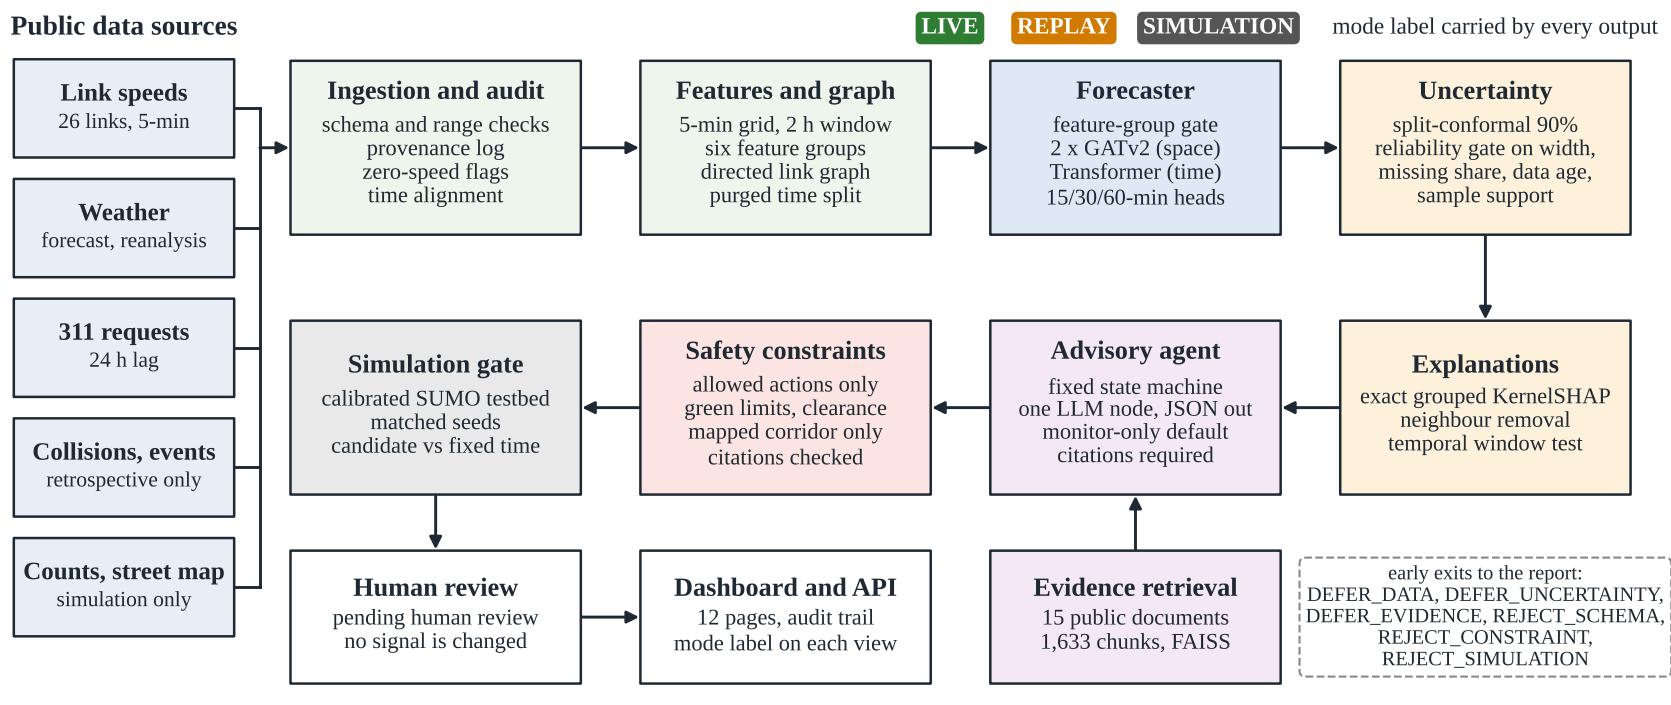
\includegraphics[width=0.978\textwidth]{fig01_architecture.png}
\caption{Architecture of the proposed system. The upper row produces calibrated forecasts; the lower row turns a reliable alert into an explained, evidence-grounded and rule-checked advisory that always ends in human review. Any failed check exits early with a named status.}
\label{fig:arch}
\end{figure*}

A traffic engineer watching a busy city grid has to decide, many times a day, whether a slowdown on one avenue will spread and whether a signal plan should change. Cities now publish road speeds, weather, service requests and incidents as open data, so the raw material for such decisions is freely available. What is missing is a way of using it that an engineer can check. A single predicted number does not say when it may be wrong, a model that gives no reasons cannot be questioned, and a language model asked for timing advice may state things that are not true unless its answer is tied to documents and held to fixed rules \cite{ji2023hallucination}.

Research on short-term traffic prediction has moved from time-series statistics to deep sequence networks and then to graph neural networks that follow the shape of the road network \cite{vlahogianni2014shortterm,jiang2022gnnsurvey}. Most of these studies measure accuracy on a few public benchmark files and report a point forecast. Much less is known about three practical questions: are the error bands honest, do the explanations reflect what the model really does, and does the model still help once it runs on a feed that arrives late? Signal control research has a gap of its own. New controllers are usually tested in a simulator, but seldom together with a forecaster that has itself been checked against real observations.

We join these pieces in a single auditable system and test each one on its own terms. Every output carries one of three labels: \textbf{LIVE} for forecasts made from the public feed before the target was observed, \textbf{REPLAY} for evaluation on held-out history, and \textbf{SIMULATION} for results from the microscopic simulator. No signal is changed in the real world; the system only advises, and every advisory ends in human review.

Fig.~\ref{fig:arch} gives an overview. The paper makes four contributions.

\noindent 1) \textbf{Context-gated graph transformer.} A forecaster that projects six feature groups into a common space, weights them with an availability-masked softmax gate, mixes information across links with two GATv2 layers and models time with a Transformer encoder, predicting 15, 30 and 60 minutes ahead.

\noindent 2) \textbf{Calibrated uncertainty with a reliability gate.} Split-conformal intervals per horizon and a gate on interval width, missing data, data age and calibration support that defers unreliable forecasts instead of passing them on.

\noindent 3) \textbf{Explainable, safety-gated agentic advisory.} A fixed state machine in which a local language model drafts a schema-checked advisory from retrieved public guidance, and deterministic constraints and a calibrated simulation gate decide what may reach a human reviewer.

\noindent 4) \textbf{Three-way evaluation with negative results kept.} A held-out test with multiple seeds and bootstrap intervals, a 45-run simulation study on a calibrated corridor, and a live test on three afternoons, in which the model did not beat persistence at short horizons.

The rest of the paper is organised as follows. Section \ref{sec:related} reviews earlier work and Section \ref{sec:data} introduces the study area and the data. Section \ref{sec:method} explains the method, Section \ref{sec:setup} the experimental setup and Section \ref{sec:results} the results. Section \ref{sec:limits} lists the limitations, and Section \ref{sec:concl} closes the paper.

\section{Related Work}\label{sec:related}
\subsection{Statistical and Deep Sequence Forecasting}
The first short-term predictors were autoregressive and Kalman-filter models. They suit steady motorway flow but cope poorly with the stop-and-go behaviour of city streets. In their review, Vlahogianni \emph{et al.} \cite{vlahogianni2014shortterm} listed the open problems of the field, among them prediction for whole networks rather than single sensors and better use of new data sources. Deep learning arrived through stacked autoencoders trained on large flow archives \cite{lv2014bigdata} and through recurrent networks; Ma \emph{et al.} \cite{ma2015lstm} found that an LSTM tracks long-range patterns in microwave-sensor speed data better than the classical methods they tried. The gated recurrent unit \cite{cho2014gru} has fewer parameters than an LSTM and is still a hard baseline to beat. Boosted tree ensembles, XGBoost \cite{chen2016xgboost} and LightGBM \cite{ke2017lightgbm}, also do well when traffic history is given to them as lag features, and they train quickly, so both serve as baselines here.

\subsection{Graph-Based Spatiotemporal Models}
Graph neural networks let the forecast for one road depend directly on the roads around it. DCRNN \cite{li2018dcrnn} describes traffic as diffusion over a directed graph and places this inside a recurrent encoder-decoder, while STGCN \cite{yu2018stgcn} drops recurrence in favour of graph and temporal convolutions. Graph WaveNet \cite{wu2019graphwavenet} learns its own adjacency matrix and pairs it with dilated convolutions, and AGCRN \cite{bai2020agcrn} learns separate parameters for each node as well as the graph. Later models lean on attention: ASTGCN \cite{guo2019astgcn} adds spatial and temporal attention to graph convolution, and GMAN \cite{zheng2020gman} builds a whole encoder-decoder from attention blocks to reach longer horizons. In graph attention networks \cite{velickovic2017gat} the weight given to each neighbour is computed from node features; GATv2 \cite{brody2022gatv2} lets the ranking of neighbours change with the node that attends to them, and it is the version used in this work. Beyond traffic, the Transformer \cite{vaswani2017attention} has largely taken over from recurrent networks for sequence data. Jiang and Luo \cite{jiang2022gnnsurvey} give a broad survey of graph models for traffic. A common thread in this literature is evaluation on fixed benchmark files, with little use of outside context or live data.

\subsection{Uncertainty Quantification}
Conformal prediction \cite{vovk2005algorithmic} builds intervals that contain the true value at a chosen rate in finite samples, as long as the data are exchangeable. Its split form needs nothing more than a separate calibration set \cite{angelopoulos2021gentle}. Traffic observed over time is not exchangeable, so the promised coverage can slip. Several remedies have been proposed: EnbPI \cite{xu2021enbpi} uses bootstrap ensembles for dynamic time series, adaptive conformal inference \cite{gibbs2021aci} moves the target miscoverage level as errors come in, and Barber \emph{et al.} \cite{barber2023beyond} bound how much coverage is lost when the distribution shifts. We keep the simple split method with one quantile per horizon and, instead of trusting its guarantee, measure where it fails.

\subsection{Explainable Machine Learning}
LIME \cite{ribeiro2016lime} explains one prediction by fitting a small, readable model around it. SHAP \cite{lundberg2017shap} brings several such methods under one framework built on Shapley values from game theory, and TreeSHAP \cite{lundberg2020treeshap} computes these values exactly for tree ensembles. Deep spatiotemporal models are harder to explain: their inputs run into the thousands, and a list of per-feature attributions is too long for an operator to read. Our approach is to group the inputs into a few meaningful blocks, compute exact Shapley values over those blocks, and test the result against two simple perturbations.

\subsection{Language-Model Agents and Retrieval}
Retrieval-augmented generation \cite{lewis2020rag} lets a language model answer from passages fetched out of a document collection. This lowers the rate of invented content but does not remove it \cite{ji2023hallucination}. Sentence embeddings \cite{reimers2019sbert} combined with a fast vector index \cite{johnson2019faiss} are the usual way to fetch those passages. Agent designs such as ReAct \cite{yao2023react} let the model decide when to reason and when to call a tool. For signal advice, where a wrong step can matter, we do the opposite: the order of steps is fixed in code, and the model is called only once, with a strict output schema.

\subsection{Signal Control and Simulation}
Signal timing practice in the United States is set out in the FHWA Signal Timing Manual \cite{fhwa2008stm} and in the MUTCD \cite{mutcd2009}. Learning-based controllers such as IntelliLight \cite{wei2018intellilight} are trained to choose phases inside a simulator, and SUMO \cite{lopez2018sumo} is a common open simulator for such work. A weakness of many of these studies is that the simulated network is never compared with measured speeds, so an apparent gain may come from the testbed rather than from the controller. In our system the simulation gate is used only after the corridor has passed a calibration against an observed speed, under a rule fixed in advance.

\subsection{Research Gap}
Table~\ref{tab:related} sets representative studies side by side with this work. We did not find an earlier study that brings together a graph forecaster trained on open city data, calibrated intervals, grouped explanations, a retrieval-backed advisory held to hard constraints, a calibrated simulation check and a live test, and that also reports which parts did not work.

\begin{table}[!t]
\caption{Comparison With Related Studies}
\label{tab:related}
\centering\scriptsize
\setlength{\tabcolsep}{3pt}
\renewcommand{\arraystretch}{1.08}
\begin{tabular}{>{\raggedright\arraybackslash}p{\dimexpr 0.2807\columnwidth-2\tabcolsep\relax}>{\centering\arraybackslash}p{\dimexpr 0.1028\columnwidth-2\tabcolsep\relax}>{\centering\arraybackslash}p{\dimexpr 0.1028\columnwidth-2\tabcolsep\relax}>{\centering\arraybackslash}p{\dimexpr 0.1028\columnwidth-2\tabcolsep\relax}>{\centering\arraybackslash}p{\dimexpr 0.1028\columnwidth-2\tabcolsep\relax}>{\centering\arraybackslash}p{\dimexpr 0.1028\columnwidth-2\tabcolsep\relax}>{\centering\arraybackslash}p{\dimexpr 0.1028\columnwidth-2\tabcolsep\relax}>{\centering\arraybackslash}p{\dimexpr 0.1028\columnwidth-2\tabcolsep\relax}}
\toprule
\textbf{Study} & \textbf{Graph} & \textbf{Multi-\newline step} & \textbf{Inter-\newline vals} & \textbf{XAI} & \textbf{LLM/\newline RAG} & \textbf{Sim.} & \textbf{Live} \\
\midrule
DCRNN \cite{li2018dcrnn} & \checkmark & \checkmark & -- & -- & -- & -- & -- \\
STGCN \cite{yu2018stgcn} & \checkmark & \checkmark & -- & -- & -- & -- & -- \\
Graph WaveNet \cite{wu2019graphwavenet} & \checkmark & \checkmark & -- & -- & -- & -- & -- \\
ASTGCN \cite{guo2019astgcn} & \checkmark & \checkmark & -- & -- & -- & -- & -- \\
GMAN \cite{zheng2020gman} & \checkmark & \checkmark & -- & -- & -- & -- & -- \\
AGCRN \cite{bai2020agcrn} & \checkmark & \checkmark & -- & -- & -- & -- & -- \\
EnbPI \cite{xu2021enbpi} & -- & -- & \checkmark & -- & -- & -- & -- \\
IntelliLight \cite{wei2018intellilight} & -- & -- & -- & -- & -- & \checkmark & -- \\
\textbf{This work} & \checkmark & \checkmark & \checkmark & \checkmark & \checkmark & \checkmark & \checkmark \\
\bottomrule
\end{tabular}
\par\vspace{2pt}
\begin{minipage}{\columnwidth}\scriptsize Multi-step: several forecast horizons. Intervals: calibrated prediction intervals. XAI: explanations of predictions. Sim.: a controller or advisory checked in a traffic simulator. Live: forecasts scored on data published after they were made.\end{minipage}
\end{table}

\section{Study Area and Data}\label{sec:data}
\subsection{Study Area}
\setcounter{figure}{1}
\begin{figure*}[!t]
\centering
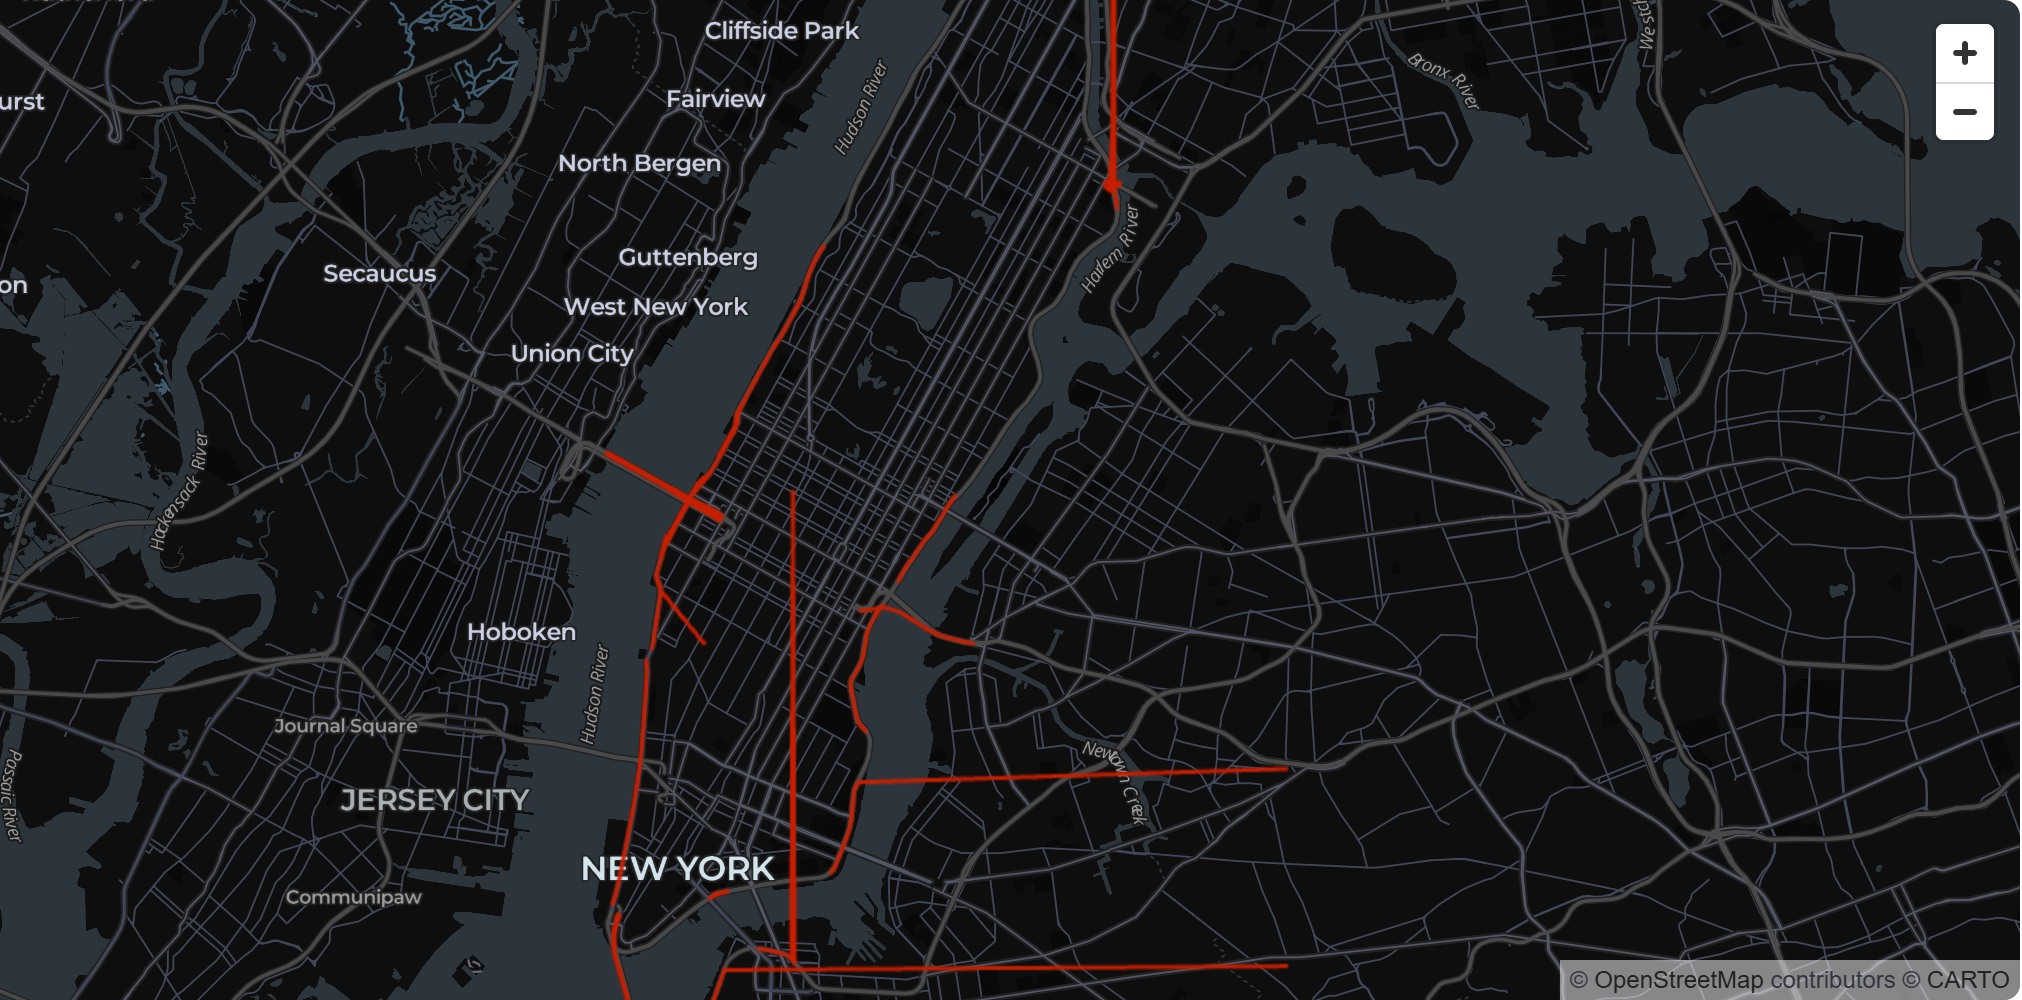
\includegraphics[width=0.850\textwidth]{fig05_study_area.png}
\caption{Monitored Manhattan road links (red) on the project dashboard map. The links cover the main avenues, the FDR Drive, the West Side Highway and the tunnel and bridge approaches.}
\label{fig:area}
\end{figure*}

The study covers Manhattan, New York City, where the city transport department publishes real-time speeds for directed road links such as avenues, the FDR Drive, the West Side Highway and tunnel and bridge approaches. Of 26 Manhattan links in the feed, seven had no valid record in 2026, leaving 19 links on the study grid. The 16 links with at least half of their training period observed enter the models (Fig.~\ref{fig:area}). A directed graph joins two links when the end of one lies within 150 m of the start of the next with a compatible heading, or when the link names state a shared endpoint; this gives 16 accepted edges, each with a recorded reason.

\subsection{Data Sources}
All inputs are public (Table~\ref{tab:sources}). Link speed is the forecasting target \cite{nycdotspeeds}. Weather comes from Open-Meteo \cite{openmeteo}: archived forecasts are used for the operational track, so the model only sees what a forecaster would have known, and reanalysis is kept for a retrospective track. Service requests (311) are used with a 24 h lag that matches their publication delay. Collisions and permitted events are published too late for operational use and are kept for retrospective analysis only. Automated volume counts \cite{nycclasscounts} and OpenStreetMap geometry are used only to build the simulation corridor.

\begin{table}[!t]
\caption{Public Data Sources}
\label{tab:sources}
\centering\footnotesize
\setlength{\tabcolsep}{3pt}
\renewcommand{\arraystretch}{1.08}
\begin{tabular}{>{\raggedright\arraybackslash}p{\dimexpr 0.3206\columnwidth-2\tabcolsep\relax}>{\raggedright\arraybackslash}p{\dimexpr 0.4739\columnwidth-2\tabcolsep\relax}>{\raggedleft\arraybackslash}p{\dimexpr 0.2055\columnwidth-2\tabcolsep\relax}}
\toprule
\textbf{Source} & \textbf{Role in this study} & \textbf{Rows used} \\
\midrule
NYC DOT link speeds \cite{nycdotspeeds} & forecast target, 26 Manhattan links & 1,968,303 \\
Open-Meteo weather \cite{openmeteo} & archived forecasts (operational); reanalysis (retrospective) & hourly \\
NYC 311 requests & infrastructure context, 24 h lag & 94,937 \\
Motor vehicle collisions & retrospective analysis only & 5,299 \\
Permitted events & retrospective analysis only & 125,617 \\
Traffic volume counts \cite{nycclasscounts} & simulation demand only & 40,492 \\
OpenStreetMap & simulation corridor geometry & extract \\
\bottomrule
\end{tabular}
\par\vspace{2pt}
\begin{minipage}{\columnwidth}\scriptsize Rows used are the Manhattan or study-window subsets downloaded for this work; every download is logged with a checksum.\end{minipage}
\end{table}

\subsection{Data Quality}
The speed feed needed heavy cleaning (Table~\ref{tab:quality}). Almost half of the raw records report a speed of zero or less, and more than half of those come from the seven links that reported zero in every record of the year; such values are treated as missing readings, not as stopped traffic, and removed, together with a handful above a plausibility limit. On the 5-minute grid, 61.1\% of the link-step cells hold a measurement, and the share varies from month to month (Fig.~\ref{fig:data}). Coverage also differs sharply between links and between the training, validation, calibration and test periods (Fig.~\ref{fig:links}); links with too little training data are kept on the grid but left out of the models.

\begin{table}[!t]
\caption{Speed Data Before and After Cleaning}
\label{tab:quality}
\centering\footnotesize
\setlength{\tabcolsep}{3pt}
\renewcommand{\arraystretch}{1.08}
\begin{tabular}{>{\raggedright\arraybackslash}p{\dimexpr 0.6712\columnwidth-2\tabcolsep\relax}>{\raggedleft\arraybackslash}p{\dimexpr 0.3288\columnwidth-2\tabcolsep\relax}}
\toprule
\textbf{Quantity} & \textbf{Value} \\
\midrule
Raw speed records & 1,968,303 \\
Zero or negative speed (removed) & 978,018 (49.7\%) \\
Above plausibility limit (removed) & 59 \\
Duplicates or unparseable times & 0 \\
Valid records kept & 990,226 (50.3\%) \\
Manhattan links in the feed & 26 \\
Links on the 5-min grid & 19 \\
Links used by the models & 16 \\
Grid time steps (5 min) & 84,084 \\
Observed share of grid cells & 61.1\% \\
Accepted directed graph edges & 16 \\
\bottomrule
\end{tabular}
\par\vspace{2pt}
\begin{minipage}{\columnwidth}\scriptsize A link enters the models when at least half of its training period is observed. Missing grid cells are masked in the loss and never scored.\end{minipage}
\end{table}

\setcounter{figure}{2}
\begin{figure}[!t]
\centering
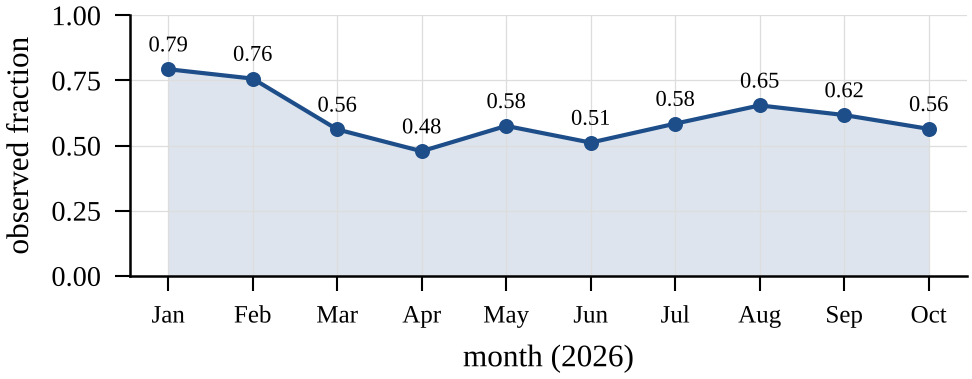
\includegraphics[width=\columnwidth]{fig19_data.png}
\caption{Monthly share of 5-minute grid cells with an observed speed on the 19 grid links (October up to the 20th).}
\label{fig:data}
\end{figure}

\setcounter{figure}{3}
\begin{figure}[!t]
\centering
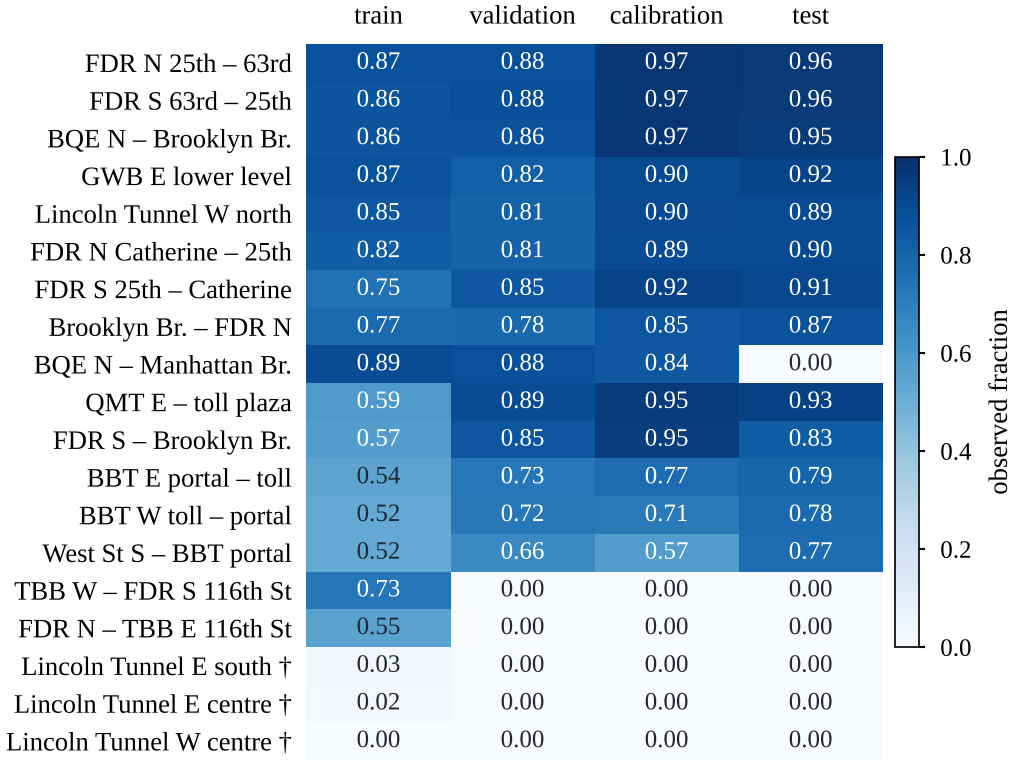
\includegraphics[width=\columnwidth]{fig20_link_heatmap.png}
\caption{Observed share of 5-minute steps for each grid link in the training, validation, calibration and test periods. Darker cells hold more data; \dag{} marks links left out of the models for too little training data.}
\label{fig:links}
\end{figure}

\subsection{Preprocessing and Quality Control}
The study window is 1 January to 20 October 2026. Each download is logged with its source, time and checksum, and a server-side audit confirms dataset identity before use. Timestamps are converted from local time to UTC, and the ambiguous daylight-saving hour is dropped instead of guessed. Of 1,968,303 raw Manhattan speed records, \textbf{978,018 report a speed of zero}, which in this feed means that no measurement was taken; these records are treated as missing and never imputed. The remaining 990,226 records are averaged onto a 5-minute grid of 84,084 steps per link, with an observed fraction of 0.611, and gaps of at most three steps are forward-filled using past values only.

\subsection{Chronological Split}
Data are split in time order into training (60\%), validation (15\%), conformal calibration (10\%) and test (15\%) partitions, with a purge gap so that no input window or target crosses a boundary. The test partition runs for 44 days, from 6 September to 20 October 2026, with 144,217, 144,213 and 144,205 valid targets at 15, 30 and 60 minutes. Three of the 16 modelled links have no valid test observation and are reported as not evaluated rather than silently dropped.

\section{Methodology}\label{sec:method}
\subsection{System Overview}
Fig.~\ref{fig:arch} shows how the parts fit together. Public data enter through an ingestion stage that audits every download, and a builder turns them into features and a link graph. The forecaster predicts speed at three horizons; each prediction receives a conformal interval and is then checked by a reliability gate. An alert that passes is explained with grouped Shapley values and handed to the advisory workflow, which fetches evidence, drafts an advisory and applies the safety rules. When a signal change is proposed, the simulation gate runs before a person reviews the result. A dashboard and an API show every stage together with its mode label.

\subsection{Problem Formulation}
Let \emph{G} = (\emph{V}, \emph{E}) be the directed link graph. At each 5-minute step \emph{t}, link \emph{v} has a feature vector \emph{x}\textsubscript{t,v} split into groups \emph{g} with availability flags \emph{m}\textsubscript{t,v,g} $\in$ {0, 1}. Given the last \emph{L} = 24 steps (two hours), the task is to predict the observed speed \emph{y}\textsubscript{t+h,v} for \emph{h} $\in$ {3, 6, 12} steps:

\begin{equation}
\hat{y}_{t+h,v} = f_{\theta}\big(X_{t-L+1:t}, G\big), \qquad h \in \{3, 6, 12\}
\end{equation}
together with an interval [\emph{$\hat{y}$} $-$ \emph{q}\textsubscript{h}, \emph{$\hat{y}$} + \emph{q}\textsubscript{h}]. An advisory may only be formed when data quality, interval width, evidence, constraints and simulation all pass; otherwise a distinct defer or reject status is returned.

\subsection{Context-Gated Graph Transformer}
The forecaster is drawn in Fig.~\ref{fig:model}. Six feature groups are used on the operational track: the link's own speed over the last 30 minutes, its speed from 30 to 120 minutes ago, the speeds of its graph neighbours, calendar terms, weather and lagged 311 counts. Each group is projected to \emph{d} = 64 dimensions, \emph{h}\textsubscript{t,v,g} = ReLU(\emph{W}\textsubscript{g}\emph{x}\textsubscript{t,v,g}). A scoring network then gives each group a weight, and groups that are missing at that step are masked out before the softmax:

\begin{equation}
\begin{aligned} \alpha_{t,v,g} &= \operatorname{softmax}_{g:\, m_{t,v,g}=1}\big(w^{\top}\tanh(U h_{t,v,g})\big), \\ z_{t,v} &= \sum_{g} \alpha_{t,v,g}\, h_{t,v,g} \end{aligned}
\end{equation}
This \textbf{availability-masked gate} lets the model keep working when a context source is late, which is common with open city data. Two \textbf{GATv2} layers with four heads, residual connections and layer normalisation then pass \emph{z} along the directed graph at every step \cite{brody2022gatv2,fey2019pyg,rozemberczki2021pgt}. Each link's sequence receives a positional embedding and enters a two-layer, four-head \textbf{Transformer encoder} (feed-forward width 128, dropout 0.1), and a linear head on the last state outputs the three horizons. The model has 158,403 parameters. Targets are standardised per link and the loss is a Huber loss averaged only over observed targets \emph{O}:

\begin{equation}
\mathcal{L}(\theta) = \frac{1}{|O|} \sum_{(t,v,h)\in O} \operatorname{Huber}_{\delta}\big(y_{t+h,v} - \hat{y}_{t+h,v}\big)
\end{equation}
\setcounter{figure}{4}
\begin{figure}[!t]
\centering
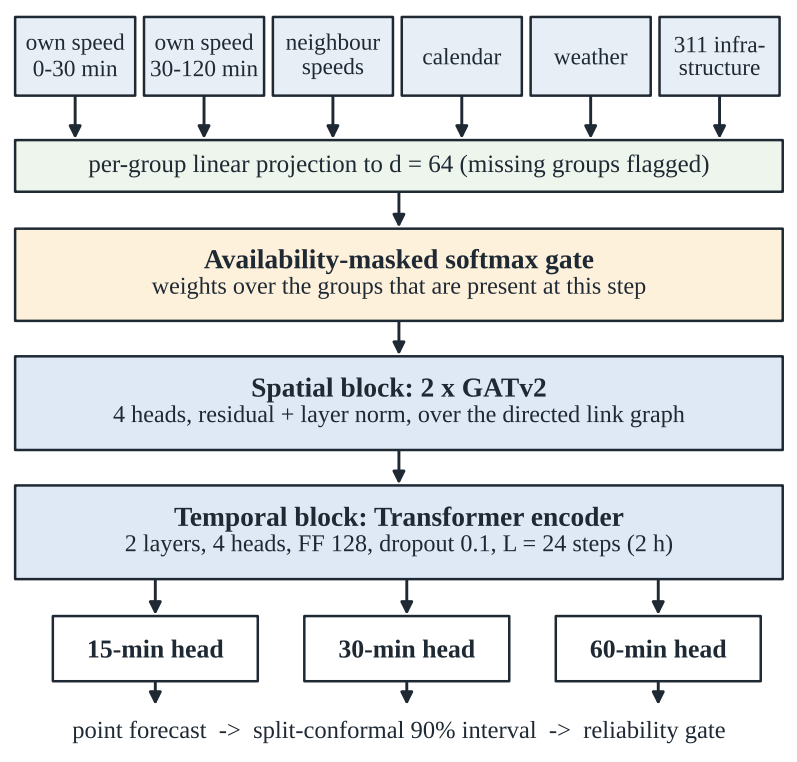
\includegraphics[width=\columnwidth]{fig02_forecaster.png}
\caption{Context-gated graph transformer. Feature groups are projected, weighted by an availability-masked gate, mixed across links by two GATv2 layers and across time by a Transformer encoder, with one head per horizon.}
\label{fig:model}
\end{figure}

\subsection{Baselines}
Six baselines share the same targets and the same mask of valid test points: persistence (last observed speed), a historical average per link, day type and 5-minute slot, XGBoost and LightGBM with one model per horizon on twelve lags and the same causal features, a GRU with 41,667 parameters, and a temporal-only Transformer that equals the proposed model without the graph layers. Ablations remove the gate (plain concatenation) or one feature group at a time.

\subsection{Conformal Intervals and Reliability Gate}
Once trained, the model is frozen, and its absolute errors on the calibration partition set the interval for each horizon. Following the split-conformal recipe \cite{angelopoulos2021gentle}, the half-width is

\begin{equation}
q_{h} = \text{the } \lceil (n+1)(1-\alpha) \rceil\text{-th smallest of } |y_{i} - \hat{y}_{i}|, \qquad \alpha = 0.1
\end{equation}
which gives half-widths of 12.1, 13.5 and 14.8 mph. The \textbf{reliability gate} defers a forecast when its interval is wider than 38.1 mph (the 80th percentile of per-link calibration widths), more than 34\% of recent inputs are missing, the newest data are older than 20 minutes, or fewer than 200 calibration samples support the link.

\subsection{Grouped Explanations}
For an alert, the quantity explained is the predicted speed in mph. The players are the six feature groups; a group that is switched off takes its values from 16 background windows drawn from the training period. Because there are only six players, all 2\textsuperscript{6} coalitions can be evaluated, so the Shapley values \cite{lundberg2017shap} are exact rather than sampled:

\begin{equation}
\varphi_{i} = \sum_{S \subseteq P \setminus \{i\}} \frac{|S|!\,(|P|-|S|-1)!}{|P|!}\,\big(v(S \cup \{i\}) - v(S)\big)
\end{equation}
Two further checks test whether the explanations agree with the model's behaviour: removing a link's graph edges, and shortening the history window from two hours down to five minutes.

\subsection{Retrieval and Agentic Advisory Workflow}
The knowledge base holds 15 public documents: the FHWA Signal Timing Manual \cite{fhwa2008stm}, two MUTCD chapters on signals \cite{mutcd2009}, nine pages of SUMO documentation and a clearly labelled project policy that lists the allowed actions. They are split into 1,633 chunks, embedded with a MiniLM sentence encoder \cite{reimers2019sbert} and indexed with FAISS \cite{johnson2019faiss}. A query whose best passage scores below a fixed threshold returns \emph{insufficient evidence}.

The workflow in Fig.~\ref{fig:flow} is a fixed state machine. Only the recommendation step calls the language model, an open-weight instruction-tuned model of about seven billion parameters that runs locally, so no data leave the machine. The model receives the forecast, interval, quality flags, attributions, retrieved passages (marked as untrusted text) and the action catalogue, and must return JSON that matches a strict schema and cites only retrieved passages. Every other step is deterministic code.

\setcounter{figure}{5}
\begin{figure}[!t]
\centering
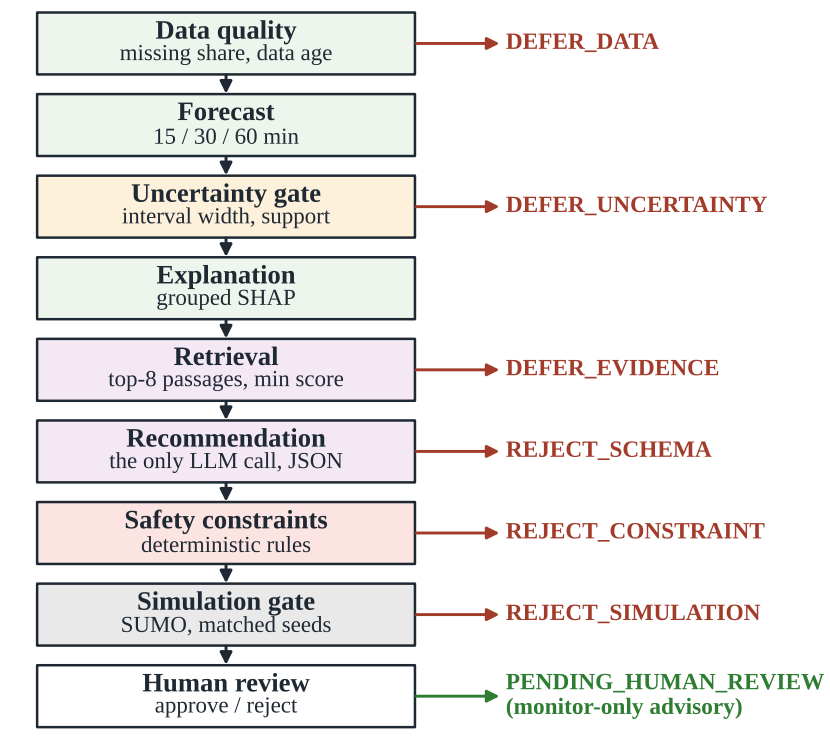
\includegraphics[width=\columnwidth]{fig03_workflow.png}
\caption{Advisory workflow. Each step can end the run with a named status; only the recommendation step uses the language model, and a completed run always waits for a human decision.}
\label{fig:flow}
\end{figure}

\subsection{Safety Constraints and Simulation Testbed}
Allowed actions are a green extension of 0 to 10 s on an existing green phase, a switch to a pre-validated program, or monitoring only. Thirteen deterministic checks cover the link-to-simulation mapping, signal and phase existence, action type, bounds, minimum and maximum green, clearance intervals, data freshness, forecast reliability and evidence support. A candidate that passes is then run in SUMO \cite{lopez2018sumo} against the fixed-time plan on matched seeds, and must cut corridor delay by at least 1\% without raising side-road delay by more than 10\% or causing any teleport.

The testbed is the West Street corridor in lower Manhattan, built from OpenStreetMap with 82 edges, 22 signals and 25 side entries, and loaded with 2025 counts of 2,510 and 2,444 vehicles per hour in the two directions \cite{nycclasscounts}. The city does not publish its timing plans, so signals start from Webster-style timing; the city's records do show that West Street was retimed for 25 mph signal progression \cite{nycvzvretiming}, which motivates the offsets tested below. Before any controller is compared, the testbed must reproduce the observed weekday evening-peak speed of 10.95 mph on the matching link within $\pm$1.5 mph, using a grid of cycle lengths, green factors and offsets fixed in advance.

\subsection{Implementation}
The system is written in Python as one package of nineteen sub-packages grouped into six layers (Fig.~\ref{fig:modules}). Typed record contracts are shared by all layers, a single command-line entry point runs every stage, and each run writes its configuration, data hashes and metrics so that every reported number can be traced back to the run that produced it. The graph layers use PyTorch Geometric \cite{fey2019pyg}, the workflow is a state graph with a human-review interrupt, and a twelve-page dashboard presents the results with their mode labels.

\setcounter{figure}{6}
\begin{figure}[!t]
\centering
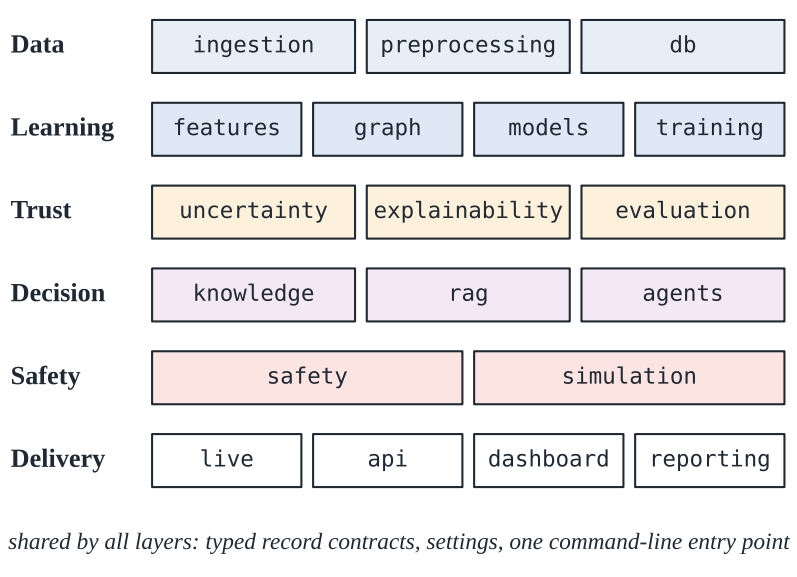
\includegraphics[width=\columnwidth]{fig04_modules.png}
\caption{Code structure of the implementation. Modules are grouped by role, from data handling to delivery; contracts and settings are shared.}
\label{fig:modules}
\end{figure}

\section{Experimental Setup}\label{sec:setup}
Table~\ref{tab:setup} lists the training settings. All learned models were trained on the same windows with early stopping on validation MAE. The main comparison uses one reference run per model; the three deep models were then retrained with seeds 1, 2 and 42 under the same budget, and differences were tested with a paired day-block bootstrap over the 44 test days. Accuracy is measured with mean absolute error (MAE), root mean squared error (RMSE) and \emph{R}\textsuperscript{2}, all in mph on observed targets only:

\begin{equation}
\mathrm{MAE} = \frac{1}{N}\sum_{i} |y_{i} - \hat{y}_{i}|, \quad \mathrm{RMSE} = \Big(\frac{1}{N}\sum_{i} (y_{i} - \hat{y}_{i})^{2}\Big)^{1/2}
\end{equation}
\begin{table}[!t]
\caption{Training and Evaluation Settings}
\label{tab:setup}
\centering\footnotesize
\setlength{\tabcolsep}{3pt}
\renewcommand{\arraystretch}{1.08}
\begin{tabular}{>{\raggedright\arraybackslash}p{\dimexpr 0.3494\columnwidth-2\tabcolsep\relax}>{\raggedright\arraybackslash}p{\dimexpr 0.6506\columnwidth-2\tabcolsep\relax}}
\toprule
\textbf{Setting} & \textbf{Value} \\
\midrule
History window \emph{L} & 24 steps (2 h), 5-min steps \\
Horizons & 3, 6, 12 steps (15/30/60 min) \\
Hidden width \emph{d} & 64 \\
Graph layers & 2 $\times$ GATv2, 4 heads, residual, layer norm \\
Temporal layers & 2 $\times$ Transformer, 4 heads, FF 128 \\
Dropout & 0.1 \\
Loss & masked Huber ($\delta$ = 1, standardised targets) \\
Optimiser & AdamW, lr 10\textsuperscript{$-$3}, weight decay 10\textsuperscript{$-$4} \\
Batch size / clipping & 8 / 1.0 \\
Epochs & $\le$ 30, early stop patience 5 \\
Windows per epoch & 4,096 sampled \\
Parameters & 158,403 (GRU: 41,667) \\
Conformal level & 90\% ($\alpha$ = 0.1), per horizon \\
Seeds & 42 (reference); 1, 2, 42 (robustness) \\
\bottomrule
\end{tabular}
\end{table}

Intervals are judged by empirical coverage against the nominal 90\% and by mean width. Retrieval is judged on 28 labelled queries by Recall@8, mean reciprocal rank (MRR) and accuracy of the supported/unsupported status. The advisory workflow is run on seven replay cases under four policies, and the simulation compares controllers on five matched seeds per scenario.

For the \textbf{live test}, forecasts were issued from the public feed after training and saved before their targets were published, then scored once the targets appeared. A strict real-time protocol could not run, because the feed published data 1.7 to 4.3 hours late, so a preregistered \emph{latest-available} protocol was used: each forecast starts from the newest bin the feed has published. The test ran on three weekday afternoons with three forecast batches each.

\section{Results and Discussion}\label{sec:results}
\subsection{Forecast Accuracy}
Table~\ref{tab:forecast} and Fig.~\ref{fig:mae} give the test errors. Every learned model beats persistence and the historical average. The proposed model has the lowest MAE at 30 and 60 minutes (5.33 and 6.15 mph), \textbf{7\%, 12\% and 16\% below persistence} at the three horizons, with \emph{R}\textsuperscript{2} of 0.69, 0.63 and 0.56 against 0.55, 0.46 and 0.30 for persistence. At 15 minutes the GRU is best (4.71 mph). The gap between persistence and the learned models grows with the horizon, which shows that recent speed alone carries most of the short-term signal while the learned context matters more further ahead.

\begin{table}[!t]
\caption{Test Error by Model and Horizon (mph, REPLAY)}
\label{tab:forecast}
\centering\scriptsize
\setlength{\tabcolsep}{3pt}
\renewcommand{\arraystretch}{1.08}
\begin{tabular}{>{\raggedright\arraybackslash}p{\dimexpr 0.2682\columnwidth-2\tabcolsep\relax}>{\raggedleft\arraybackslash}p{\dimexpr 0.1220\columnwidth-2\tabcolsep\relax}>{\raggedleft\arraybackslash}p{\dimexpr 0.1220\columnwidth-2\tabcolsep\relax}>{\raggedleft\arraybackslash}p{\dimexpr 0.1220\columnwidth-2\tabcolsep\relax}>{\raggedleft\arraybackslash}p{\dimexpr 0.1220\columnwidth-2\tabcolsep\relax}>{\raggedleft\arraybackslash}p{\dimexpr 0.1220\columnwidth-2\tabcolsep\relax}>{\raggedleft\arraybackslash}p{\dimexpr 0.1220\columnwidth-2\tabcolsep\relax}}
\toprule
\textbf{Model} & \multicolumn{2}{c}{15 min} & \multicolumn{2}{c}{30 min} & \multicolumn{2}{c}{60 min} \\
\cmidrule(lr){2-3} \cmidrule(lr){4-5} \cmidrule(lr){6-7}
 & \textbf{MAE} & \textbf{RMSE} & \textbf{MAE} & \textbf{RMSE} & \textbf{MAE} & \textbf{RMSE} \\
\midrule
Persistence & 5.14 & 9.14 & 6.06 & 10.05 & 7.29 & 11.43 \\
Historical average & 7.63 & 10.48 & 7.63 & 10.49 & 7.64 & 10.49 \\
XGBoost & 4.82 & 7.62 & 5.58 & 8.35 & 6.31 & 8.98 \\
LightGBM & 4.87 & 7.72 & 5.60 & 8.35 & 6.32 & 9.03 \\
GRU & \textbf{4.71} & 7.55 & 5.37 & 8.26 & 6.17 & 9.03 \\
Temporal Transf. & 4.73 & 7.62 & 5.34 & 8.31 & 6.18 & 9.12 \\
\textbf{Proposed} & 4.77 & 7.63 & \textbf{5.33} & 8.28 & \textbf{6.15} & 9.05 \\
\bottomrule
\end{tabular}
\par\vspace{2pt}
\begin{minipage}{\columnwidth}\scriptsize Held-out test period of 44 days; \emph{n} = 144,217, 144,213 and 144,205 valid targets. Same mask for all models; reference run with seed 42. Bold: lowest MAE.\end{minipage}
\end{table}

\setcounter{figure}{7}
\begin{figure}[!t]
\centering
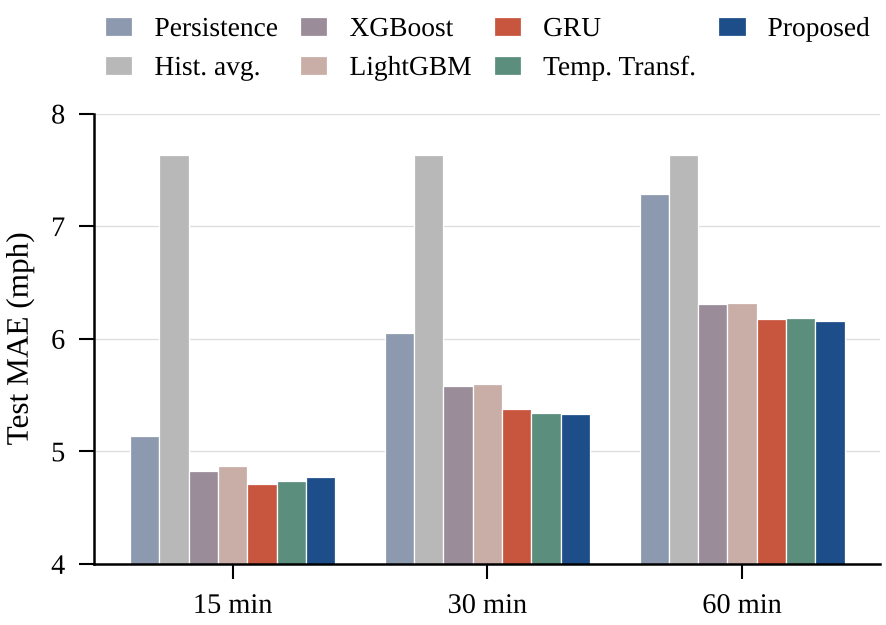
\includegraphics[width=\columnwidth]{fig06_mae.png}
\caption{Test MAE of all models at the three horizons (REPLAY). The vertical axis starts at 4 mph to make the differences between learned models visible.}
\label{fig:mae}
\end{figure}

\subsection{Robustness Across Seeds}
A single run can flatter a model, so the three deep models were retrained with three seeds (Table~\ref{tab:seeds}, Fig.~\ref{fig:seeds}). The proposed model is significantly better than the temporal Transformer at every horizon, which credits the graph layers, but its edge over the GRU is small: the GRU is better at 15 minutes (difference $-$0.021 mph, 95\% interval [$-$0.040, $-$0.004]) and worse at 30 and 60 minutes by about 0.03 mph. \textbf{The accuracy gain is therefore real but small}, and a simpler recurrent model remains a fair choice for the shortest horizon. The graph layers use non-deterministic scatter operations, so runs with the same seed are not bit-identical; the later stages all use the seed-42 reference model.

\begin{table}[!t]
\caption{Test MAE Over Three Seeds (mph)}
\label{tab:seeds}
\centering\scriptsize
\setlength{\tabcolsep}{3pt}
\renewcommand{\arraystretch}{1.08}
\begin{tabular}{>{\raggedright\arraybackslash}p{\dimexpr 0.2643\columnwidth-2\tabcolsep\relax}>{\centering\arraybackslash}p{\dimexpr 0.2454\columnwidth-2\tabcolsep\relax}>{\centering\arraybackslash}p{\dimexpr 0.2454\columnwidth-2\tabcolsep\relax}>{\centering\arraybackslash}p{\dimexpr 0.2450\columnwidth-2\tabcolsep\relax}}
\toprule
\textbf{Model} & \textbf{15 min} & \textbf{30 min} & \textbf{60 min} \\
\midrule
Proposed & 4.688 $\pm$ 0.063 & 5.339 $\pm$ 0.032 & 6.153 $\pm$ 0.015 \\
GRU & 4.666 $\pm$ 0.057 & 5.370 $\pm$ 0.020 & 6.184 $\pm$ 0.010 \\
Temporal Transf. & 4.723 $\pm$ 0.032 & 5.375 $\pm$ 0.033 & 6.233 $\pm$ 0.075 \\
$\Delta$ GRU & $-$0.021\newline [$-$0.040, $-$0.004] & +0.032\newline [+0.010, +0.052] & +0.031\newline [+0.007, +0.056] \\
$\Delta$ Temporal Transf. & +0.035\newline [+0.019, +0.051] & +0.037\newline [+0.018, +0.054] & +0.080\newline [+0.054, +0.104] \\
\bottomrule
\end{tabular}
\par\vspace{2pt}
\begin{minipage}{\columnwidth}\scriptsize Mean $\pm$ standard deviation over seeds 1, 2 and 42. $\Delta$ rows: model minus proposed, with a 95\% paired day-block bootstrap interval; positive values favour the proposed model.\end{minipage}
\end{table}

\setcounter{figure}{8}
\begin{figure}[!t]
\centering
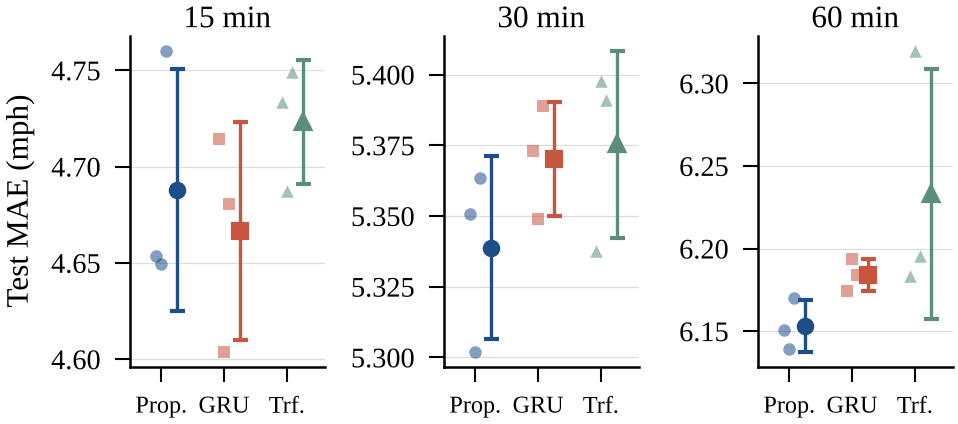
\includegraphics[width=\columnwidth]{fig07_seeds.png}
\caption{Test MAE over seeds 1, 2 and 42. Small markers are single runs; large markers show the mean and one standard deviation.}
\label{fig:seeds}
\end{figure}

\subsection{Ablation and Sensitivity}
Removing the availability gate raises the mean MAE by 0.067 mph (95\% interval [0.048, 0.086]) and removing the 311 group by 0.014 mph, so both help slightly (Table~\ref{tab:ablation}, Fig.~\ref{fig:ablation}a). Removing weather, however, \textbf{lowers} the error by 0.046 mph: on this test period the weather forecasts added noise rather than signal, and we report this as a negative finding. Shortening the history window raises the error steadily, from 5.43 mph with two hours to 7.11 mph with five minutes (Fig.~\ref{fig:ablation}b), so the model does use its full window.

\setcounter{figure}{9}
\begin{figure}[!t]
\centering
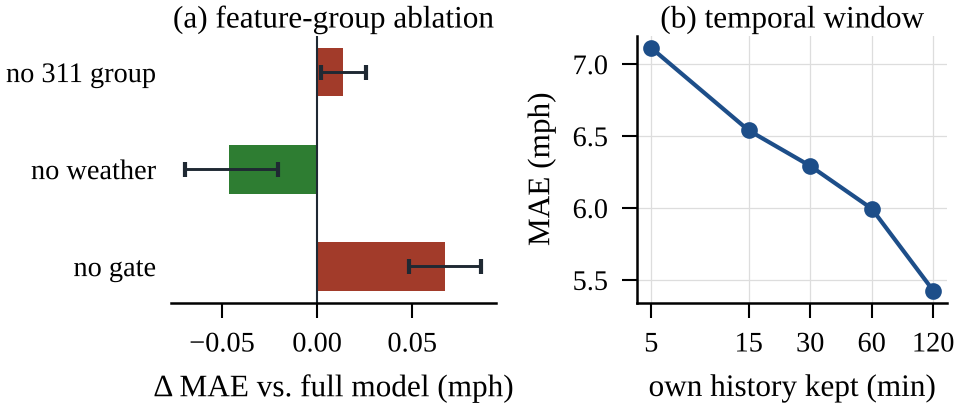
\includegraphics[width=\columnwidth]{fig08_ablation_window.png}
\caption{(a) Change in mean test MAE when a component is removed, with 95\% day-block bootstrap intervals. (b) MAE when the link's own history is cut to shorter windows.}
\label{fig:ablation}
\end{figure}

\begin{table}[!t]
\caption{Ablation and History-Window Sensitivity (Test MAE, mph)}
\label{tab:ablation}
\centering\footnotesize
\setlength{\tabcolsep}{3pt}
\renewcommand{\arraystretch}{1.08}
\begin{tabular}{>{\raggedright\arraybackslash}p{\dimexpr 0.3835\columnwidth-2\tabcolsep\relax}>{\raggedleft\arraybackslash}p{\dimexpr 0.1644\columnwidth-2\tabcolsep\relax}>{\raggedleft\arraybackslash}p{\dimexpr 0.1726\columnwidth-2\tabcolsep\relax}>{\centering\arraybackslash}p{\dimexpr 0.2795\columnwidth-2\tabcolsep\relax}}
\toprule
\textbf{Variant} & \textbf{MAE} & \textbf{$\Delta$ MAE} & \textbf{95\% interval} \\
\midrule
\multicolumn{4}{@{}l@{}}{\emph{(a) Component removed, mean over horizons}} \\
Proposed (reference) & 5.419 & -- & -- \\
No availability gate & 5.487 & +0.067 & [0.048, 0.086] \\
No weather group & 5.373 & $-$0.046 & [$-$0.069, $-$0.021] \\
No 311 group & 5.433 & +0.014 & [0.002, 0.026] \\
No events group & -- & -- & not applicable \\
No incidents group & -- & -- & not applicable \\
\multicolumn{4}{@{}l@{}}{\emph{(b) Own history kept, reference model}} \\
2 h (full window) & 5.427 & -- & -- \\
1 h & 5.997 & +0.569 & -- \\
30 min & 6.293 & +0.866 & -- \\
15 min & 6.540 & +1.113 & -- \\
5 min & 7.113 & +1.686 & -- \\
\bottomrule
\end{tabular}
\par\vspace{2pt}
\begin{minipage}{\columnwidth}\scriptsize $\Delta$: variant minus reference; positive values mean the removed part helped. Intervals from a paired day-block bootstrap over 44 test days. Events and incidents are not available in time for operational use, so those ablations do not apply.\end{minipage}
\end{table}

\subsection{Uncertainty and the Reliability Gate}
The conformal intervals reach 0.909, 0.907 and 0.903 coverage at the three horizons, close to the nominal 0.90 (Table~\ref{tab:unc}). Coverage is not uniform, though (Fig.~\ref{fig:unc}a). It is about 0.93 in free flow and moderate traffic but falls to \textbf{0.80, 0.79 and 0.76 in congestion}, exactly where advice matters most, because the intervals have one width per horizon. Rush hours (0.93 to 0.94) and wet periods (0.92 to 0.93) are slightly over-covered. The reliability gate defers about a quarter of forecasts; on the retained ones the MAE falls to 3.72, 4.38 and 5.25 mph and coverage rises to 0.93 to 0.95 (Fig.~\ref{fig:unc}b). The gate thus trades coverage of the network for reliability of what is passed on.

\begin{table}[!t]
\caption{Conformal Intervals and Reliability Gate (REPLAY)}
\label{tab:unc}
\centering\scriptsize
\setlength{\tabcolsep}{3pt}
\renewcommand{\arraystretch}{1.08}
\begin{tabular}{>{\raggedright\arraybackslash}p{\dimexpr 0.1534\columnwidth-2\tabcolsep\relax}>{\raggedleft\arraybackslash}p{\dimexpr 0.1411\columnwidth-2\tabcolsep\relax}>{\raggedleft\arraybackslash}p{\dimexpr 0.1411\columnwidth-2\tabcolsep\relax}>{\raggedleft\arraybackslash}p{\dimexpr 0.1411\columnwidth-2\tabcolsep\relax}>{\raggedleft\arraybackslash}p{\dimexpr 0.1411\columnwidth-2\tabcolsep\relax}>{\raggedleft\arraybackslash}p{\dimexpr 0.1411\columnwidth-2\tabcolsep\relax}>{\raggedleft\arraybackslash}p{\dimexpr 0.1411\columnwidth-2\tabcolsep\relax}}
\toprule
\textbf{Horizon} & \textbf{Half-\newline width} & \textbf{Cover-\newline age} & \textbf{Cov.\newline congested} & \textbf{Deferred\newline (\%)} & \textbf{MAE\newline retained} & \textbf{Cov.\newline retained} \\
\midrule
15 min & 12.1 & 0.909 & 0.798 & 25.5 & 3.72 & 0.948 \\
30 min & 13.5 & 0.907 & 0.794 & 25.7 & 4.38 & 0.939 \\
60 min & 14.8 & 0.903 & 0.757 & 26.1 & 5.25 & 0.930 \\
\bottomrule
\end{tabular}
\par\vspace{2pt}
\begin{minipage}{\columnwidth}\scriptsize Nominal coverage 0.90. Half-width in mph. Congested: speed below half of free flow. Retained: forecasts that pass the reliability gate.\end{minipage}
\end{table}

\setcounter{figure}{10}
\begin{figure}[!t]
\centering
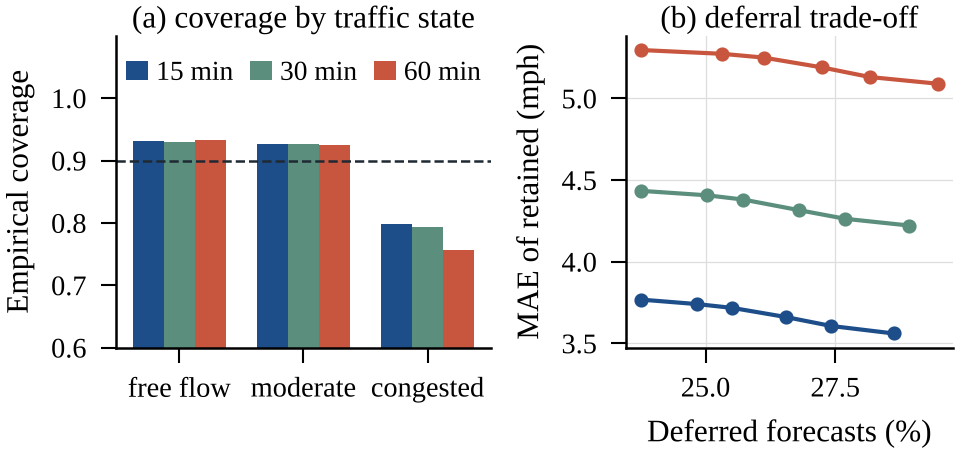
\includegraphics[width=\columnwidth]{fig09_uncertainty.png}
\caption{(a) Empirical coverage of the 90\% intervals by traffic state and horizon (nominal level 0.90). (b) MAE of retained forecasts against the share deferred, for the gate's missing-data threshold.}
\label{fig:unc}
\end{figure}

\subsection{Explanations}
Across twelve explained alerts, the link's own last 30 minutes dominate the attributions (mean absolute value 8.22 mph), followed by its older history (2.04), calendar (1.09) and neighbours (0.52), with weather (0.19) and 311 (0.09) close to zero (Table~\ref{tab:xai}, Fig.~\ref{fig:shap}a). This agrees with the ablation, in which weather did not help. In one alert on a bridge approach the model predicted 2.25 mph against a background of 26.9 mph (observed 1.24 mph), and the recent-history group accounted for $-$21.3 mph of that drop, a reading an operator can check against the raw series. Removing a link's graph edges changes its predictions by 0.67 to 1.34 mph, and not at all for the West Street link. The LightGBM baseline, explained with TreeSHAP, gives a similar ranking (Fig.~\ref{fig:shap}b): traffic lags take 72\%, 64\% and 52\% of the attribution at 15, 30 and 60 minutes, and calendar terms gain weight with the horizon (18\%, 24\% and 34\%).

\setcounter{figure}{11}
\begin{figure}[!t]
\centering
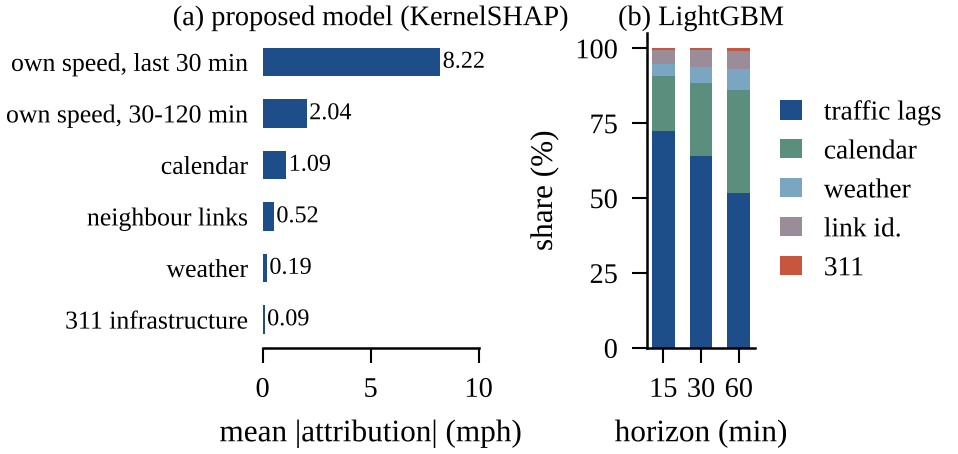
\includegraphics[width=\columnwidth]{fig10_shap.png}
\caption{(a) Mean absolute grouped Shapley value of the proposed model over twelve alerts. (b) Share of TreeSHAP attribution by group for the LightGBM baseline at each horizon.}
\label{fig:shap}
\end{figure}

\begin{table}[!t]
\caption{Grouped Attributions of the Forecasts}
\label{tab:xai}
\centering\footnotesize
\setlength{\tabcolsep}{3pt}
\renewcommand{\arraystretch}{1.08}
\begin{tabular}{>{\raggedright\arraybackslash}p{\dimexpr 0.3753\columnwidth-2\tabcolsep\relax}>{\raggedleft\arraybackslash}p{\dimexpr 0.1808\columnwidth-2\tabcolsep\relax}>{\centering\arraybackslash}p{\dimexpr 0.2219\columnwidth-2\tabcolsep\relax}>{\centering\arraybackslash}p{\dimexpr 0.2219\columnwidth-2\tabcolsep\relax}}
\toprule
\textbf{Feature group} & \textbf{Mean |\emph{$\varphi$}|\newline (mph)} & \textbf{Share (\%)} & \textbf{Largest in\newline alerts} \\
\midrule
Own speed, last 30 min & 8.22 & 67.7 & 8 of 12 \\
Own speed, 30--120 min & 2.04 & 16.8 & 4 of 12 \\
Calendar & 1.09 & 9.0 & 0 of 12 \\
Graph neighbours & 0.52 & 4.3 & 0 of 12 \\
Weather & 0.19 & 1.6 & 0 of 12 \\
311 requests & 0.09 & 0.7 & 0 of 12 \\
\multicolumn{4}{@{}l@{}}{\emph{LightGBM, TreeSHAP share (\%) at 15 / 30 / 60 min}} \\
Traffic lags &  & 72 / 64 / 52 &  \\
Calendar &  & 18 / 24 / 34 &  \\
Weather &  & 4 / 5 / 7 &  \\
311 requests &  & 0 / 1 / 1 &  \\
Link identity &  & 5 / 6 / 6 &  \\
\bottomrule
\end{tabular}
\par\vspace{2pt}
\begin{minipage}{\columnwidth}\scriptsize Proposed model: exact grouped KernelSHAP over 12 alerts (half the largest drops, half random). Attributions describe model sensitivity, not causes on the street.\end{minipage}
\end{table}

\subsection{Retrieval and Advisory Workflow}
\setcounter{figure}{12}
\begin{figure*}[!t]
\centering
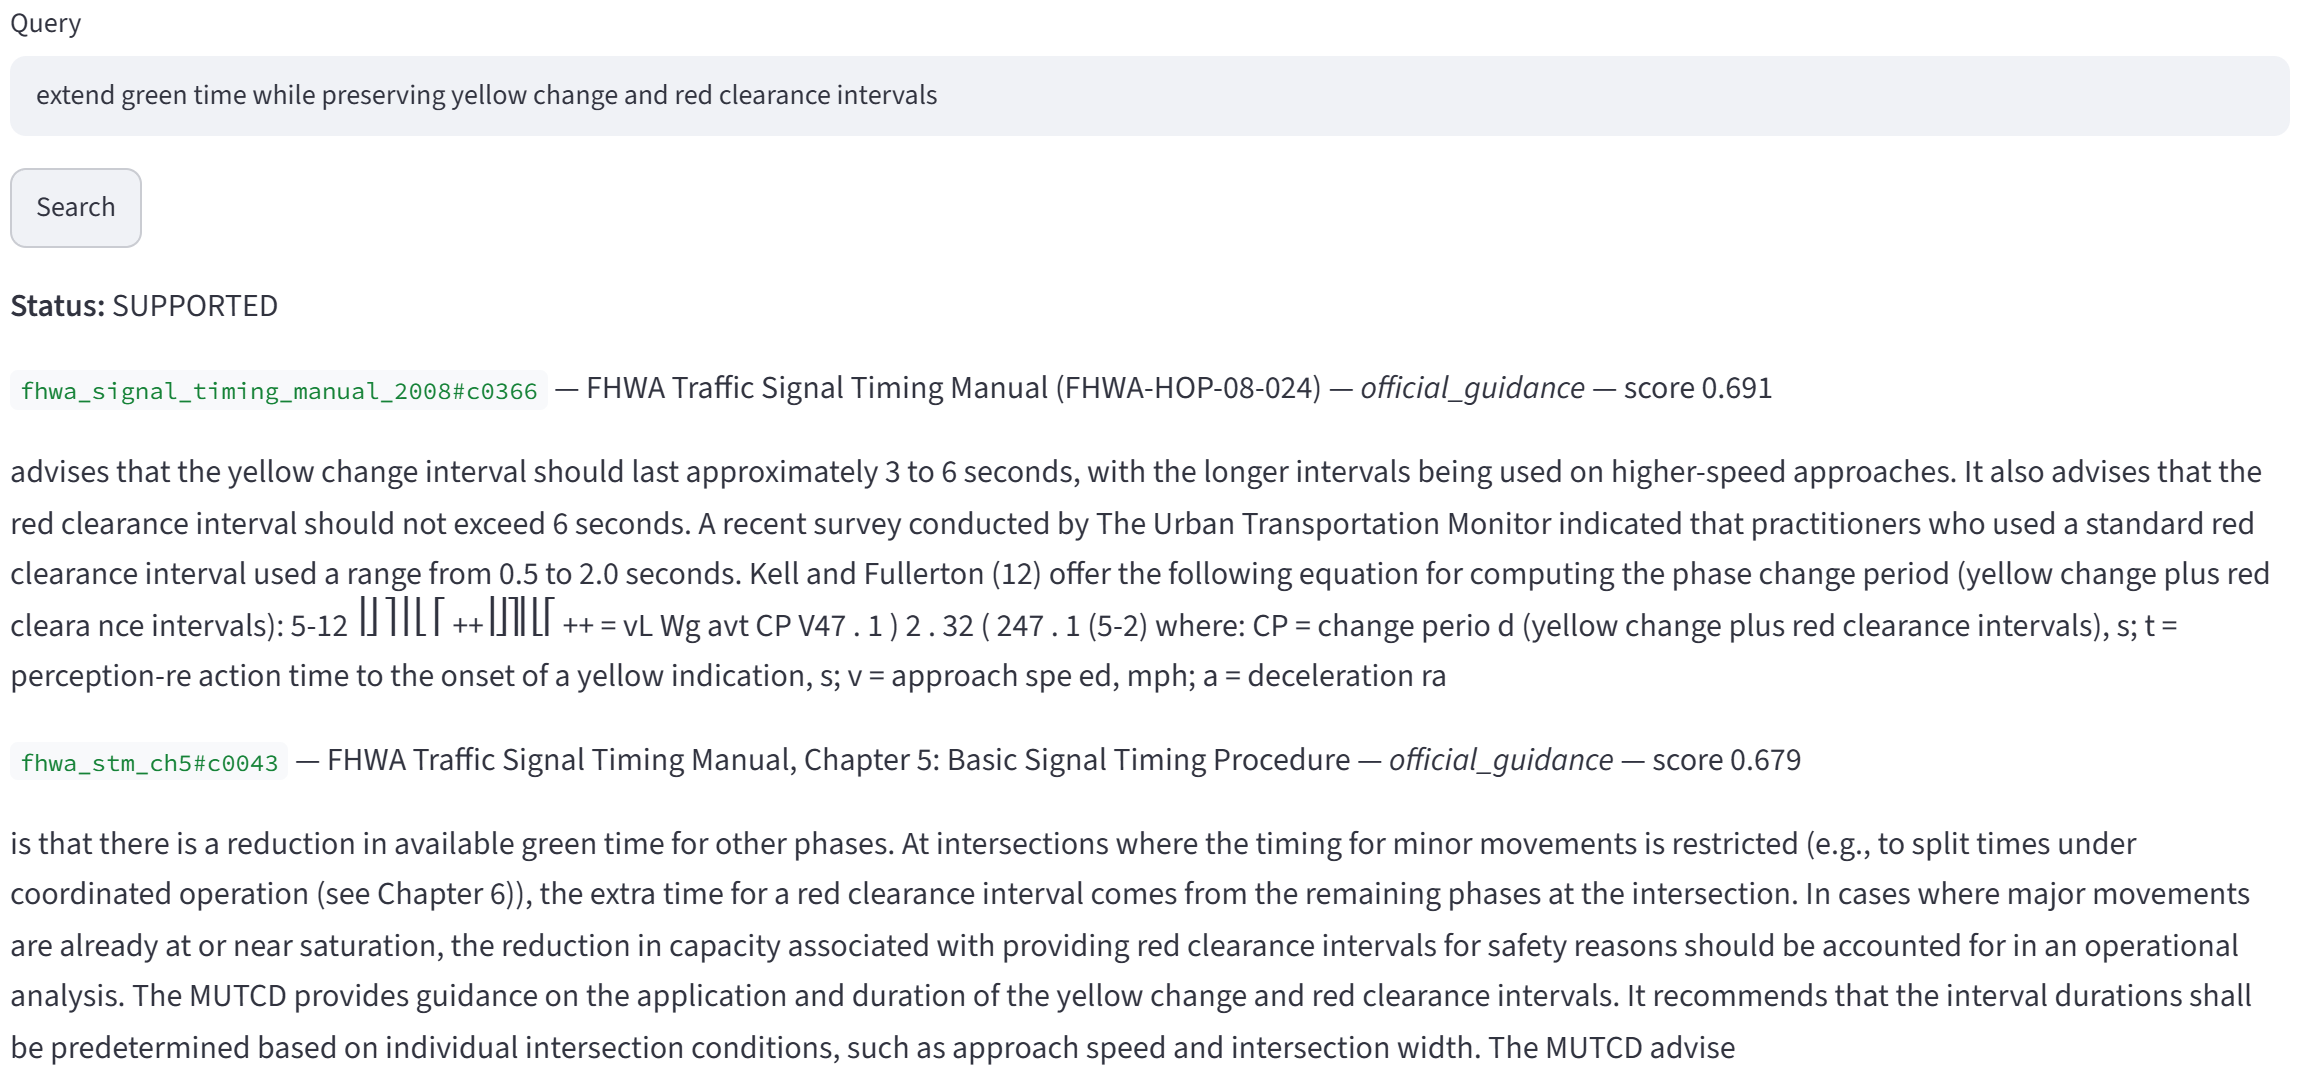
\includegraphics[width=0.978\textwidth]{fig16_dash_retrieval.png}
\caption{Evidence retrieval page of the dashboard: a query about signal timing returns ranked passages from the public manuals, each with its source and similarity score.}
\label{fig:retshot}
\end{figure*}

\setcounter{figure}{13}
\begin{figure*}[!t]
\centering
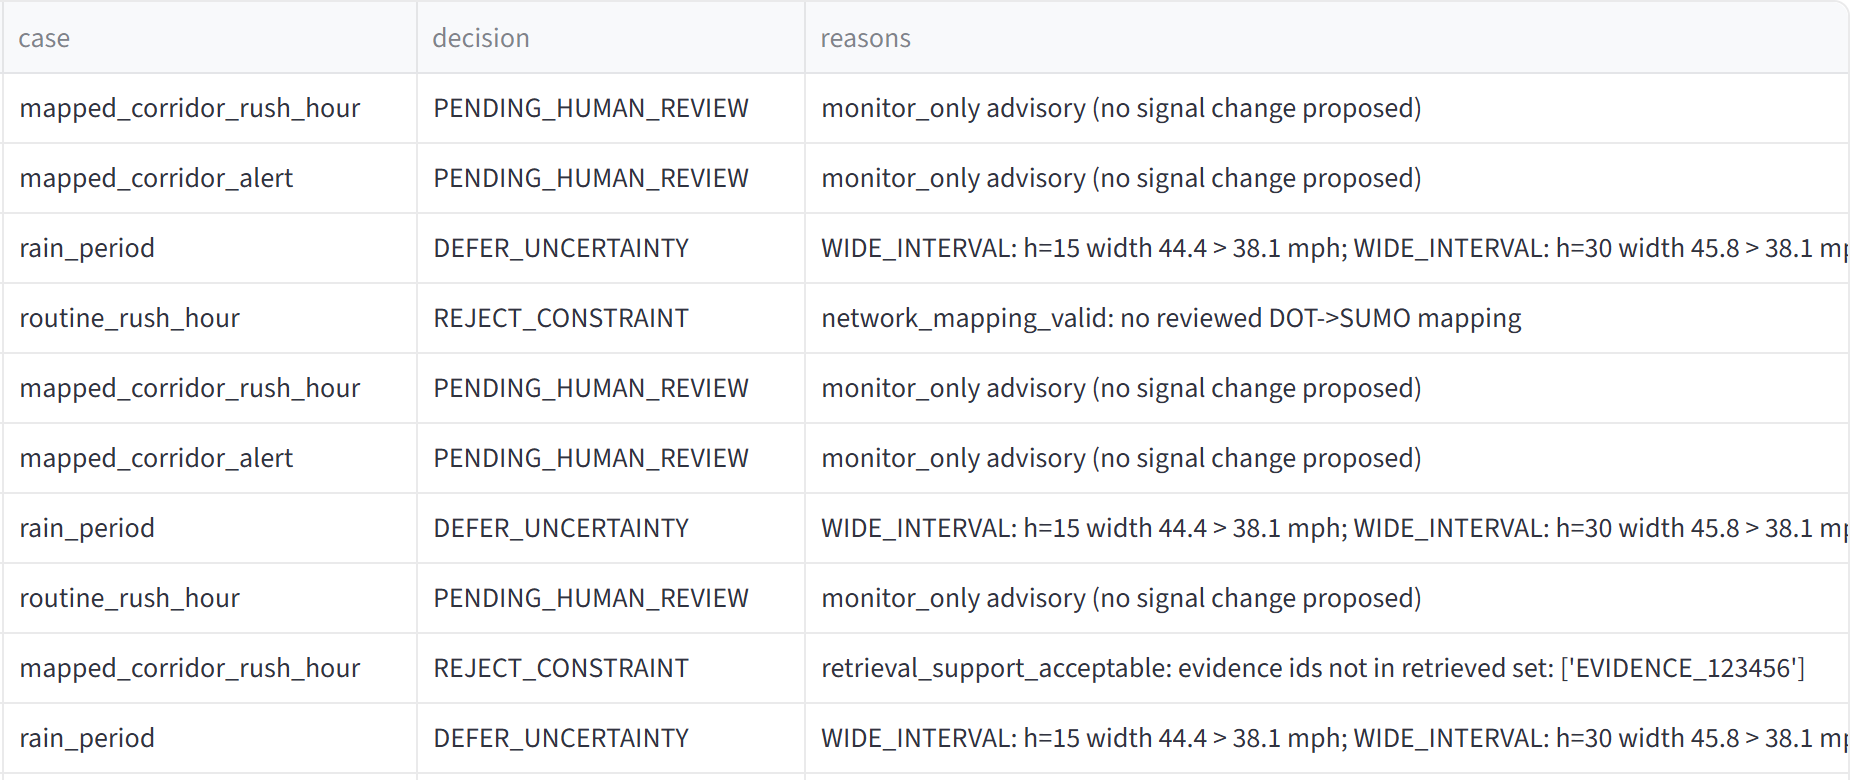
\includegraphics[width=0.978\textwidth]{fig17_dash_agent.png}
\caption{Audit table of advisory runs on the dashboard (REPLAY). Each run records its case, its final decision and the reasons, such as a wide interval, a missing network mapping or an invented evidence identifier.}
\label{fig:agent}
\end{figure*}

On 28 labelled queries, retrieval reaches \textbf{Recall@8 of 0.841} and an MRR of 0.748, and the supported/unsupported status is right for 27 of 28 queries (0.964) (Table~\ref{tab:retrieval}). The one error is an out-of-scope query whose best passage scored 0.45, above the evidence threshold of 0.35. The labels were reviewed by the first author and not by an independent annotator, which limits how far these figures can be generalised. Fig.~\ref{fig:retshot} shows a retrieval result as the operator sees it.

\begin{table}[!t]
\caption{Retrieval Evaluation on 28 Labelled Queries}
\label{tab:retrieval}
\centering\footnotesize
\setlength{\tabcolsep}{3pt}
\renewcommand{\arraystretch}{1.08}
\begin{tabular}{>{\raggedright\arraybackslash}p{\dimexpr 0.6712\columnwidth-2\tabcolsep\relax}>{\raggedleft\arraybackslash}p{\dimexpr 0.3288\columnwidth-2\tabcolsep\relax}}
\toprule
\textbf{Measure} & \textbf{Value} \\
\midrule
Documents / chunks & 15 / 1,633 \\
Chunks cut at the encoder limit & 171 \\
Embedding size & 384 \\
Labelled queries (answerable / out of scope) & 28 (22 / 6) \\
Recall@8 (answerable) & 0.841 \\
Mean reciprocal rank (answerable) & 0.748 \\
Correct status, all queries & 27 of 28 (0.964) \\
Out-of-scope queries refused & 5 of 6 \\
Evidence threshold (cosine) & 0.35 \\
Median query time (s) & 0.028 \\
\bottomrule
\end{tabular}
\par\vspace{2pt}
\begin{minipage}{\columnwidth}\scriptsize Labels reviewed by the first author, not by an independent annotator. Query time excludes the first query, which also loads the encoder.\end{minipage}
\end{table}

Table~\ref{tab:adv} summarises 19 advisory runs (seven cases under the full system and four under each of three reduced policies), repeated in three passes with 36 language-model calls in total. Every call returned valid JSON and every pass reached the same 19 decisions. Without retrieval, the model invented an evidence identifier in all three cases where it drafted an advisory, and the citation check rejected each one; with retrieval, none of nine drafts cited a missing passage. Without the constraint layer, an advisory for a link that has no mapping to the simulator reached human review, whereas the full system rejected it. In the full system, wide intervals, stale data and missing evidence ended runs early as intended, and the two corridor cases ended as monitor-only advisories pending human review. \textbf{No real advisory reached the simulation gate}, so the gate has only been exercised by the controller study below. In the latest pass a language-model call took 18 to 54 s, so an advisory that reached a draft took 23 to 59 s end to end, while runs that ended early took under 6 s. Fig.~\ref{fig:agent} shows the audit table in which each run is listed with its recorded reasons.

\begin{table}[!t]
\caption{Advisory Outcomes by Policy (REPLAY)}
\label{tab:adv}
\centering\scriptsize
\setlength{\tabcolsep}{3pt}
\renewcommand{\arraystretch}{1.08}
\begin{tabular}{>{\raggedright\arraybackslash}p{\dimexpr 0.3424\columnwidth-2\tabcolsep\relax}>{\raggedleft\arraybackslash}p{\dimexpr 0.1151\columnwidth-2\tabcolsep\relax}>{\raggedleft\arraybackslash}p{\dimexpr 0.1397\columnwidth-2\tabcolsep\relax}>{\raggedleft\arraybackslash}p{\dimexpr 0.1315\columnwidth-2\tabcolsep\relax}>{\raggedleft\arraybackslash}p{\dimexpr 0.1315\columnwidth-2\tabcolsep\relax}>{\raggedleft\arraybackslash}p{\dimexpr 0.1397\columnwidth-2\tabcolsep\relax}}
\toprule
\textbf{Policy} & \textbf{Runs} & \textbf{Pending\newline review} & \textbf{Deferred} & \textbf{Rejected} & \textbf{Invalid\newline citations} \\
\midrule
Full system & 7 & 2 & 4 & 1 & 0 \\
Without retrieval & 4 & 0 & 1 & 3 & 3 \\
Without constraints & 4 & 3 & 1 & 0 & 0 \\
Without simulation gate & 4 & 2 & 1 & 1 & 0 \\
\bottomrule
\end{tabular}
\par\vspace{2pt}
\begin{minipage}{\columnwidth}\scriptsize Identical decisions in each of three passes. Pending review advisories are monitor-only; no signal change was proposed.\end{minipage}
\end{table}

\subsection{Simulation Calibration}
The testbed did not match reality at first. With Webster-style timing the corridor ran at 5.82 mph against the observed 10.95 mph, and scaling the green split alone never rose above 8.22 mph (Fig.~\ref{fig:calib}, Table~\ref{tab:calib}). A common 90 s cycle reached 8.88 mph, and adding offsets for a 25 mph southbound platoon brought it to \textbf{10.08 mph, inside the $\pm$1.5 mph band}; this cell (green factor 1.5) was selected by the preregistered rule. A 120 s cycle overshot to 13.1 to 21.7 mph. The calibrated network is a scenario testbed tuned to one speed on one link, not a model of the city's actual timing plans. An earlier version of the testbed wrote demand as origin-destination flows, which the simulator re-routes on current travel times \cite{sumodocs_routing}, so part of the traffic left the corridor; an audit found this, and all runs reported here use fixed free-flow routes on the corridor.

\begin{table}[!t]
\caption{Calibration Grid Summary (SIMULATION)}
\label{tab:calib}
\centering\scriptsize
\setlength{\tabcolsep}{3pt}
\renewcommand{\arraystretch}{1.08}
\begin{tabular}{>{\raggedright\arraybackslash}p{\dimexpr 0.2067\columnwidth-2\tabcolsep\relax}>{\centering\arraybackslash}p{\dimexpr 0.1315\columnwidth-2\tabcolsep\relax}>{\centering\arraybackslash}p{\dimexpr 0.1891\columnwidth-2\tabcolsep\relax}>{\centering\arraybackslash}p{\dimexpr 0.2137\columnwidth-2\tabcolsep\relax}>{\raggedleft\arraybackslash}p{\dimexpr 0.1356\columnwidth-2\tabcolsep\relax}>{\centering\arraybackslash}p{\dimexpr 0.1233\columnwidth-2\tabcolsep\relax}}
\toprule
\textbf{Timing family} & \textbf{Admis-\newline sible} & \textbf{Speed range\newline (mph)} & \textbf{Closest: factor\newline / speed} & \textbf{Gap\newline (mph)} & \textbf{In\newline band} \\
\midrule
Webster & 3 of 5 & 5.82--8.22 & 3.0 / 8.22 & $-$2.73 & no \\
90 s & 4 of 5 & 6.79--8.88 & 1.5 / 8.88 & $-$2.07 & no \\
\textbf{90 s + offsets} & \textbf{4 of 5} & \textbf{7.88--10.08} & \textbf{1.5 / 10.08} & \textbf{$-$0.87} & \textbf{yes} \\
120 s & 4 of 5 & 7.16--13.11 & 1.5 / 13.11 & +2.16 & no \\
120 s + offsets & 5 of 5 & 8.22--21.67 & 1.0 / 8.22 & $-$2.73 & no \\
\bottomrule
\end{tabular}
\par\vspace{2pt}
\begin{minipage}{\columnwidth}\scriptsize Five green factors (1.0 to 3.0) per family, three seeds each. Target: observed 10.95 mph $\pm$ 1.5 on the mapped link. Admissible: no teleport and at most 1\% unfinished trips in every seed. Bold: the family of the selected cell.\end{minipage}
\end{table}

\subsection{Controller Comparison in Simulation}
On the calibrated corridor, three controllers were run in three scenarios with five matched seeds, 45 runs in all, none with a teleport (Table~\ref{tab:sim}, Fig.~\ref{fig:ctrl}). The forecast rule extends corridor green by 5 s when the forecast flags congestion. In the routine peak it is never triggered, so it equals fixed time (271.6 s time loss per trip). Under the event surge it lowers time loss from 450.2 s to 426.0 s (\textbf{$-$5.4\%}) and completes 5,910 trips instead of 5,720; in the incident scenario time loss falls from 465.9 s to 443.9 s (\textbf{$-$4.7\%}) with 5,919 trips completed instead of 5,725. The rule wins in every seed, by 12.9 to 33.7 s, and it is not a survivorship effect, because more trips finish rather than fewer. The actuated controller uses the simulator's own uncalibrated programs and is shown only as a reference. These are simulation results on a calibrated scenario testbed without side-street demand or pedestrians; they are \textbf{not evidence of a real-world gain}.

\setcounter{figure}{14}
\begin{figure}[!t]
\centering
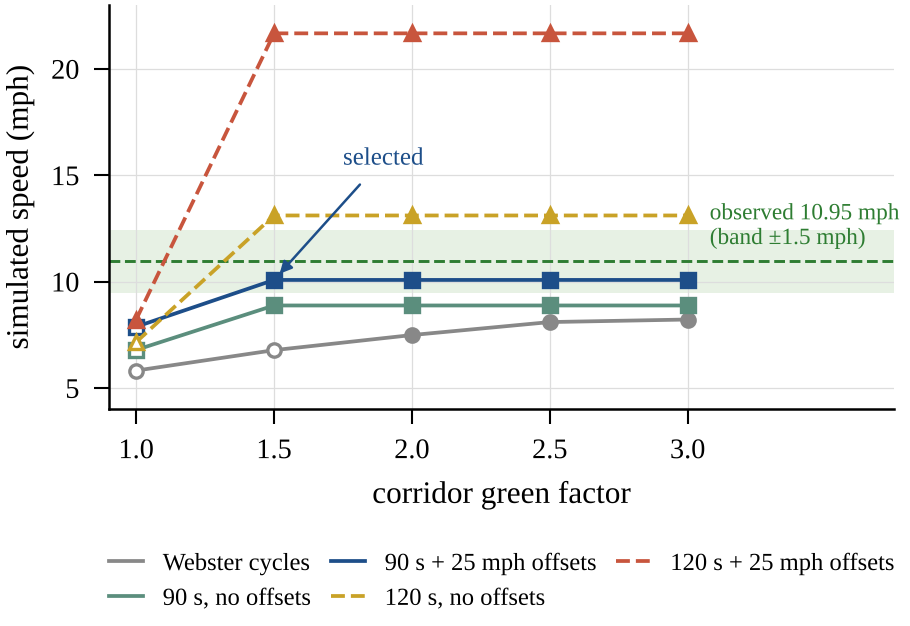
\includegraphics[width=\columnwidth]{fig11_calibration.png}
\caption{Calibration of the SUMO corridor (SIMULATION): mean simulated speed on the mapped link against the green factor for each timing family. Filled markers are admissible cells; the band is the observed speed $\pm$1.5 mph.}
\label{fig:calib}
\end{figure}

\begin{table}[!t]
\caption{Controller Comparison on the Calibrated Corridor (SIMULATION)}
\label{tab:sim}
\centering\scriptsize
\setlength{\tabcolsep}{3pt}
\renewcommand{\arraystretch}{1.08}
\begin{tabular}{>{\raggedright\arraybackslash}p{\dimexpr 0.1808\columnwidth-2\tabcolsep\relax}>{\raggedright\arraybackslash}p{\dimexpr 0.2137\columnwidth-2\tabcolsep\relax}>{\raggedleft\arraybackslash}p{\dimexpr 0.1562\columnwidth-2\tabcolsep\relax}>{\raggedleft\arraybackslash}p{\dimexpr 0.1574\columnwidth-2\tabcolsep\relax}>{\raggedleft\arraybackslash}p{\dimexpr 0.1562\columnwidth-2\tabcolsep\relax}>{\raggedleft\arraybackslash}p{\dimexpr 0.1356\columnwidth-2\tabcolsep\relax}}
\toprule
\textbf{Scenario} & \textbf{Controller} & \textbf{Time loss\newline (s/trip)} & \textbf{Completed} & \textbf{Unfinished} & \textbf{Max\newline queue} \\
\midrule
Routine & Fixed time & 271.6 & 4,975 & 0 & 292 \\
 & Forecast rule & 271.6 & 4,975 & 0 & 292 \\
Event surge & Fixed time & 450.2 & 5,720 & 540 & 368 \\
 & Forecast rule & 426.0 & 5,910 & 350 & 358 \\
Incident & Fixed time & 465.9 & 5,725 & 536 & 385 \\
 & Forecast rule & 443.9 & 5,919 & 341 & 367 \\
\bottomrule
\end{tabular}
\par\vspace{2pt}
\begin{minipage}{\columnwidth}\scriptsize Mean over five matched seeds; no teleports. Uncalibrated actuated reference: routine 384.8 s, event surge 538.2 s, incident 554.4 s.\end{minipage}
\end{table}

\setcounter{figure}{15}
\begin{figure}[!t]
\centering
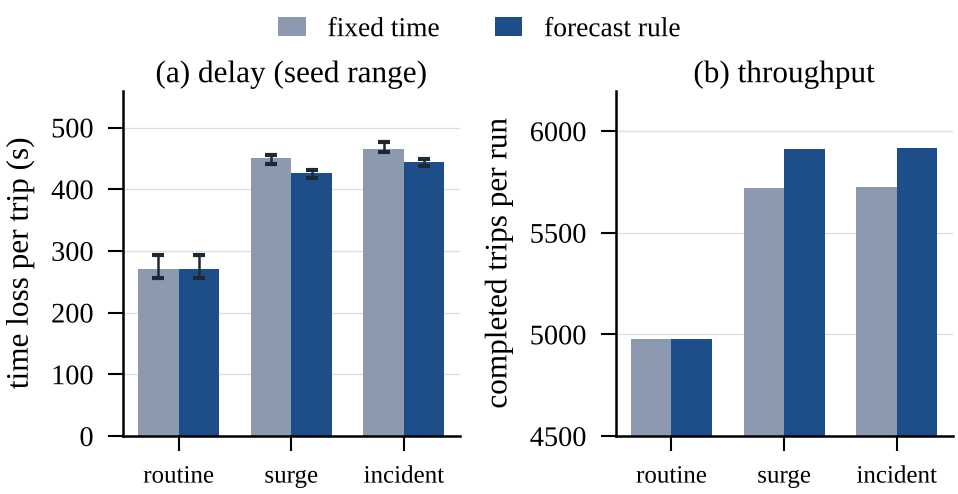
\includegraphics[width=\columnwidth]{fig12_controllers.png}
\caption{Fixed time against the forecast-triggered rule on the calibrated corridor (SIMULATION, five seeds). (a) Time loss per completed trip with the range over seeds. (b) Completed trips per run.}
\label{fig:ctrl}
\end{figure}

\subsection{Live Test}
\setcounter{figure}{18}
\begin{figure*}[!t]
\centering
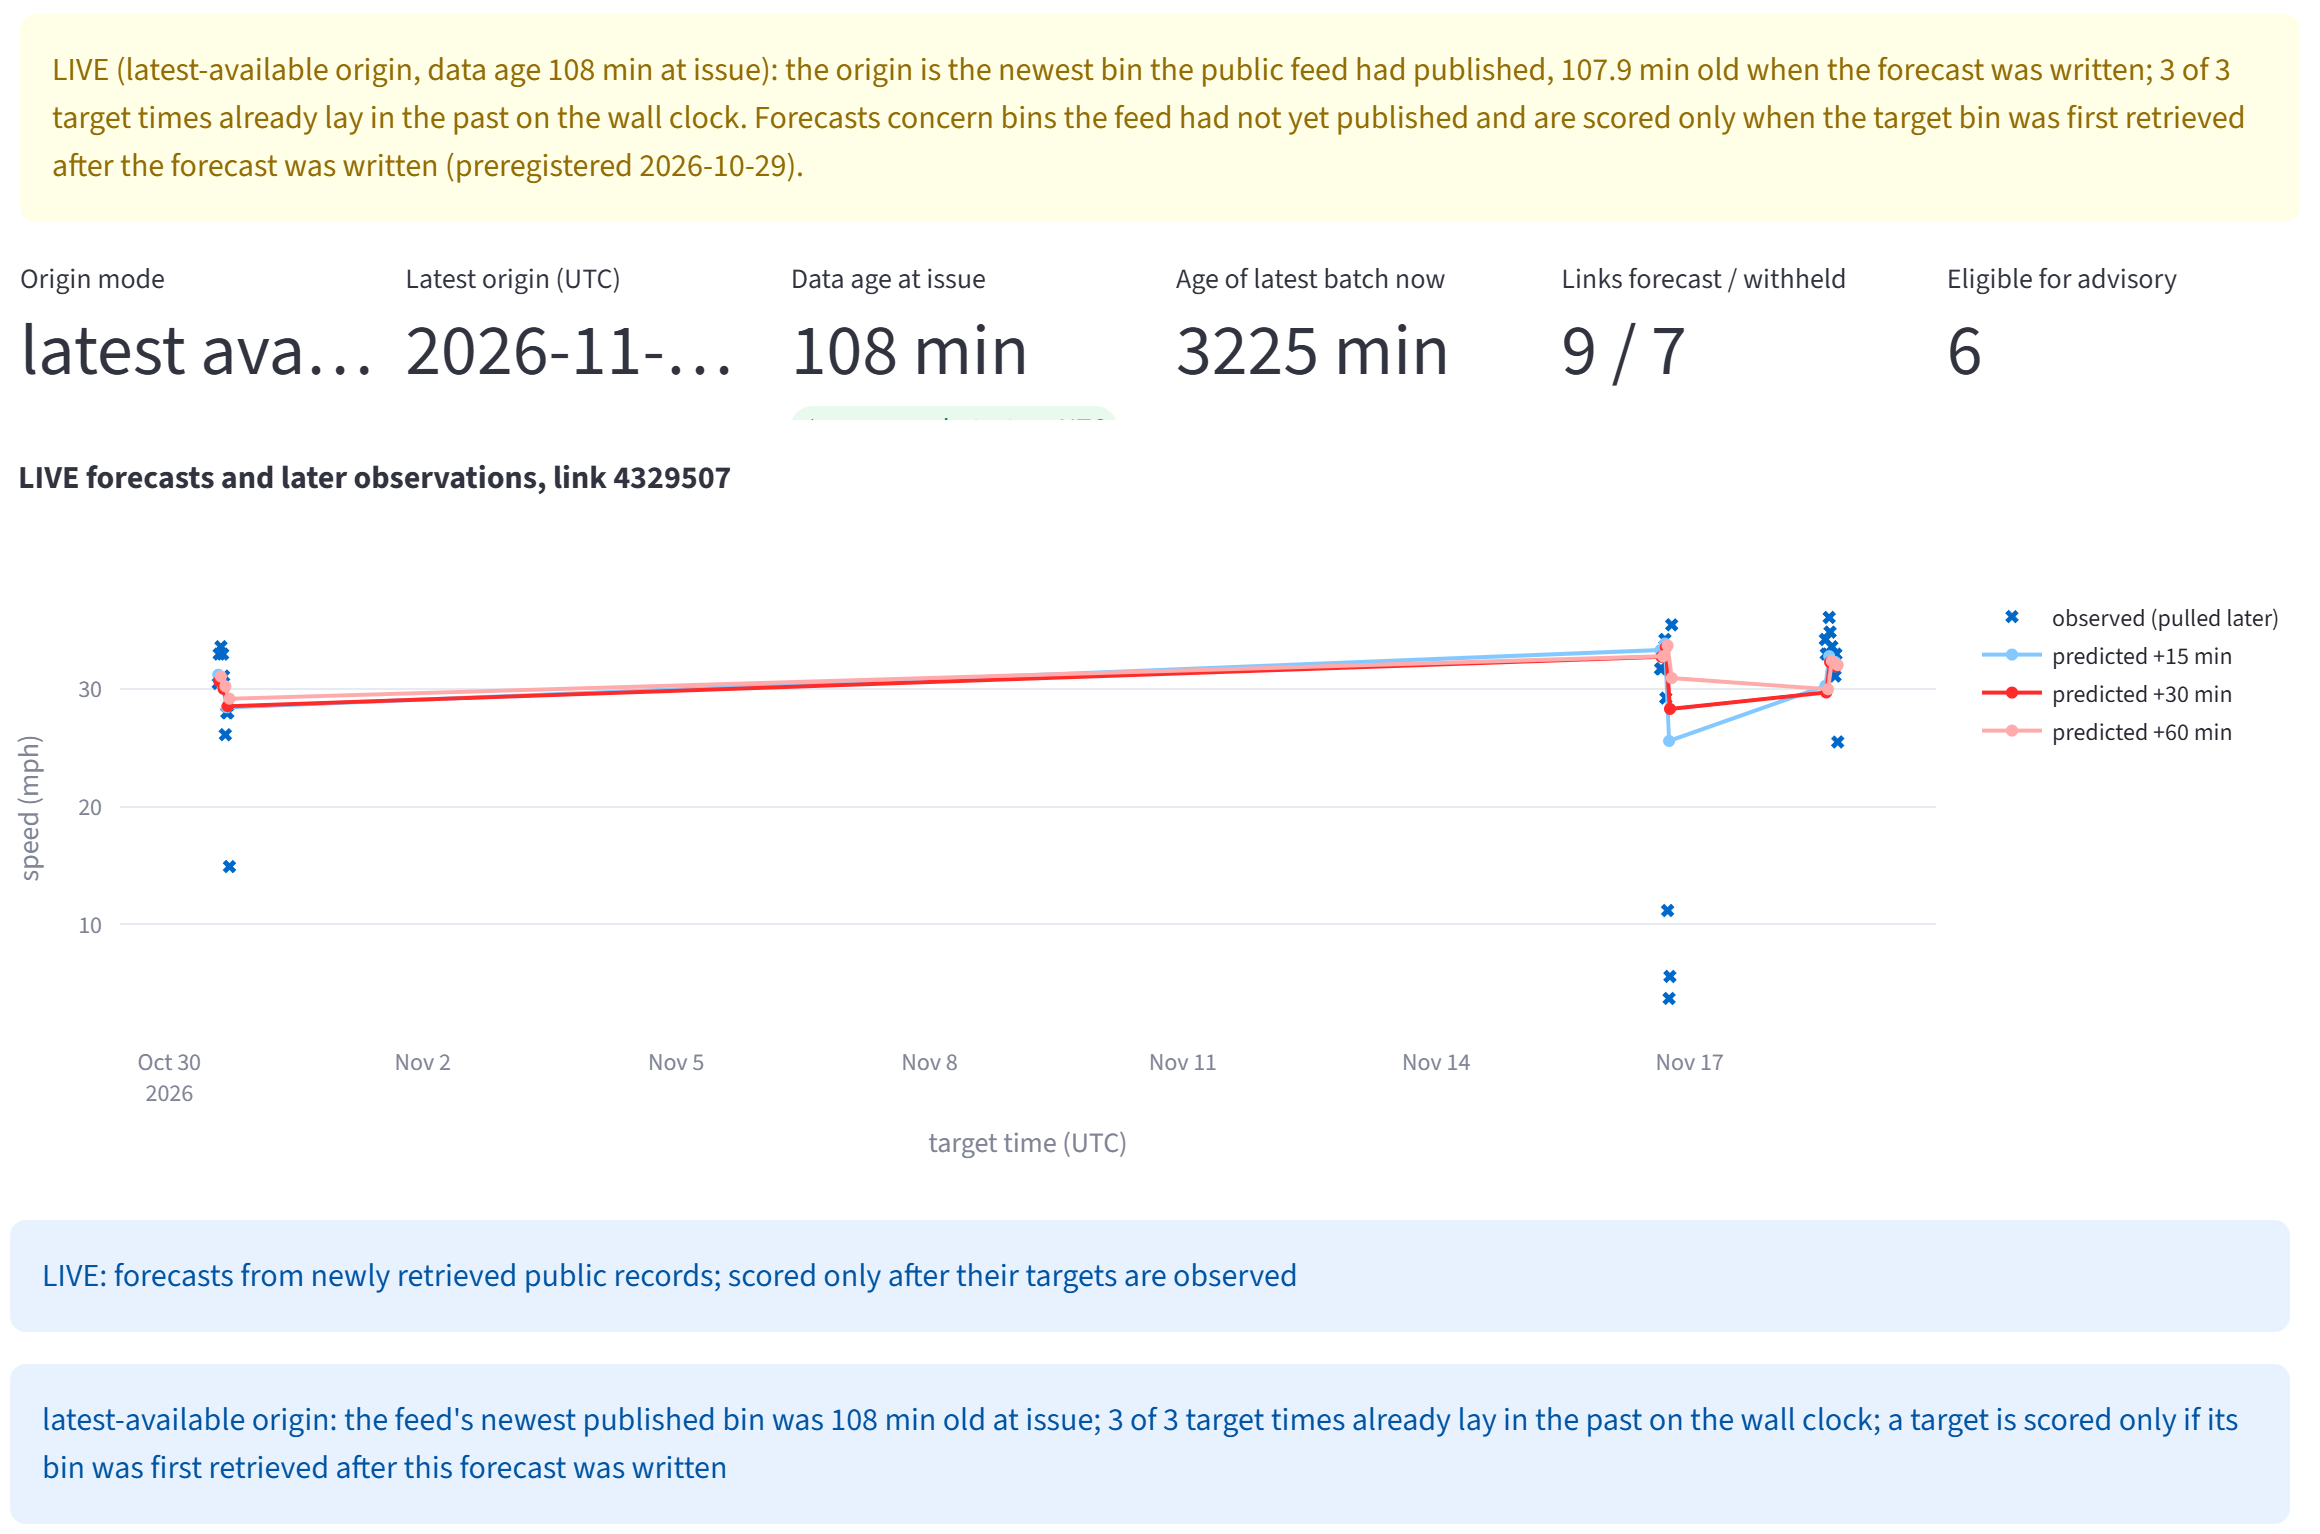
\includegraphics[width=0.922\textwidth]{fig18_dash_live.png}
\caption{Live monitoring page of the dashboard (LIVE). Top: the protocol banner with the data age of the latest batch. Middle: live forecasts of one link at 15, 30 and 60 minutes against the observations pulled later. Bottom: the labels that every live batch carries.}
\label{fig:liveshot}
\end{figure*}

Table~\ref{tab:live} and Fig.~\ref{fig:live} give the live results. On the first afternoon the model beat persistence at all three horizons. On the second it lost at 15 and 30 minutes, and on the third it lost at every horizon. Pooled over 274 scored forecasts (two of 276 targets were never published), the MAE is 4.79, 4.94 and 5.48 mph against 4.63, 4.42 and 5.46 mph for persistence: \textbf{persistence is ahead at 15 and 30 minutes and level at 60 minutes}. Coverage held up better, at 0.880, 0.901 and 0.912. The forecasts started from data that were on average 100 to 130 minutes old, and at that age the most recent observed speed is a hard baseline to beat. Restricted to the links eligible for advice, the model's MAE is lower (3.88, 4.22 and 4.70 mph), but with nine afternoon batches this is not a second test set. \textbf{The test-set gain did not carry over to the live feed at its present delay}, and we report this as the main live finding.

\begin{table}[!t]
\caption{Live Forecast Error, Model / Persistence (mph, LIVE)}
\label{tab:live}
\centering\scriptsize
\setlength{\tabcolsep}{3pt}
\renewcommand{\arraystretch}{1.08}
\begin{tabular}{>{\raggedright\arraybackslash}p{\dimexpr 0.1233\columnwidth-2\tabcolsep\relax}>{\raggedleft\arraybackslash}p{\dimexpr 0.1028\columnwidth-2\tabcolsep\relax}>{\raggedleft\arraybackslash}p{\dimexpr 0.1110\columnwidth-2\tabcolsep\relax}>{\raggedleft\arraybackslash}p{\dimexpr 0.0904\columnwidth-2\tabcolsep\relax}>{\centering\arraybackslash}p{\dimexpr 0.1907\columnwidth-2\tabcolsep\relax}>{\centering\arraybackslash}p{\dimexpr 0.1907\columnwidth-2\tabcolsep\relax}>{\centering\arraybackslash}p{\dimexpr 0.1911\columnwidth-2\tabcolsep\relax}}
\toprule
\textbf{After-\newline noon} & \textbf{Links} & \textbf{Age\newline (min)} & \textbf{\emph{n}} & \textbf{15 min} & \textbf{30 min} & \textbf{60 min} \\
\midrule
A1 & 13 & 114 & 39 & 3.62 / 4.25 & 5.50 / 6.17 & 5.25 / 5.59 \\
A2 & 9 & 100 & 27 & 4.94 / 4.05 & 4.52 / 3.54 & 5.65 / 5.78 \\
A3 & 9 & 129 & 26 & 6.37 / 5.79 & 4.52 / 2.63 & 5.65 / 4.90 \\
Pooled & -- & 114 & 92 & \textbf{4.79} / \textbf{4.63} & \textbf{4.94} / \textbf{4.42} & \textbf{5.48} / \textbf{5.46} \\
\bottomrule
\end{tabular}
\par\vspace{2pt}
\begin{minipage}{\columnwidth}\scriptsize Latest-available origin; age is the mean data age when the forecast was issued; \emph{n} at 15 min (the pooled 30 and 60 min rows have 91). Pooled coverage of the 90\% intervals: 0.880, 0.901 and 0.912.\end{minipage}
\end{table}

\setcounter{figure}{16}
\begin{figure}[!t]
\centering
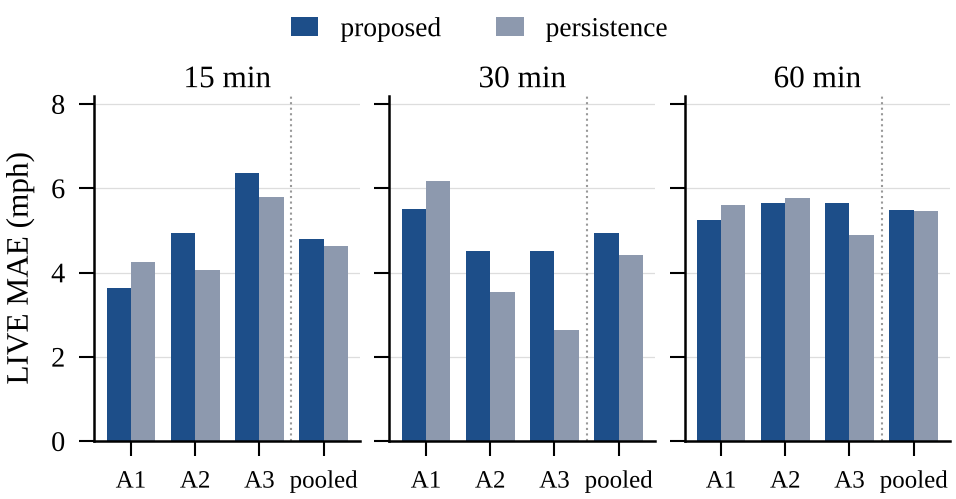
\includegraphics[width=\columnwidth]{fig13_live.png}
\caption{Live MAE of the proposed model and of persistence on three afternoons (A1 to A3) and pooled (LIVE, latest-available origin).}
\label{fig:live}
\end{figure}

Fig.~\ref{fig:livescatter} looks at the individual forecasts. Both the model and persistence follow the observed speeds and their error distributions are similar in shape, but the model's median and 90th-percentile errors are slightly larger (3.25 and 12.3 mph against 3.11 and 11.2 mph), which is enough to put persistence ahead on the pooled MAE. Fig.~\ref{fig:liveshot} shows how the dashboard reports the live batches with their data age and labels.

\setcounter{figure}{17}
\begin{figure}[!t]
\centering
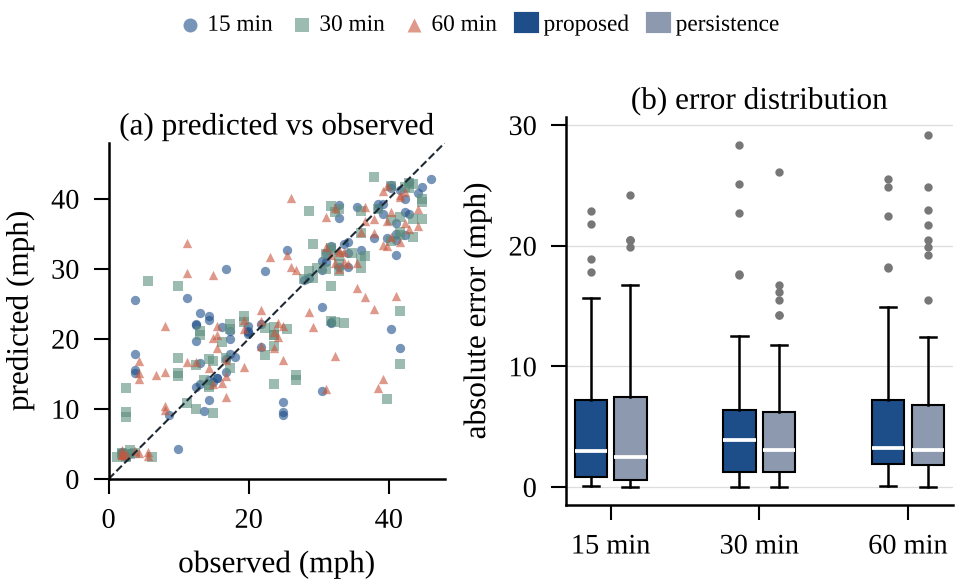
\includegraphics[width=\columnwidth]{fig23_live_scatter.png}
\caption{(a) Predicted against observed speed for all 274 scored live forecasts. (b) Absolute error of the model and of persistence at each horizon (LIVE).}
\label{fig:livescatter}
\end{figure}

\subsection{Dashboard and Run Time}
\setcounter{figure}{19}
\begin{figure*}[!t]
\centering
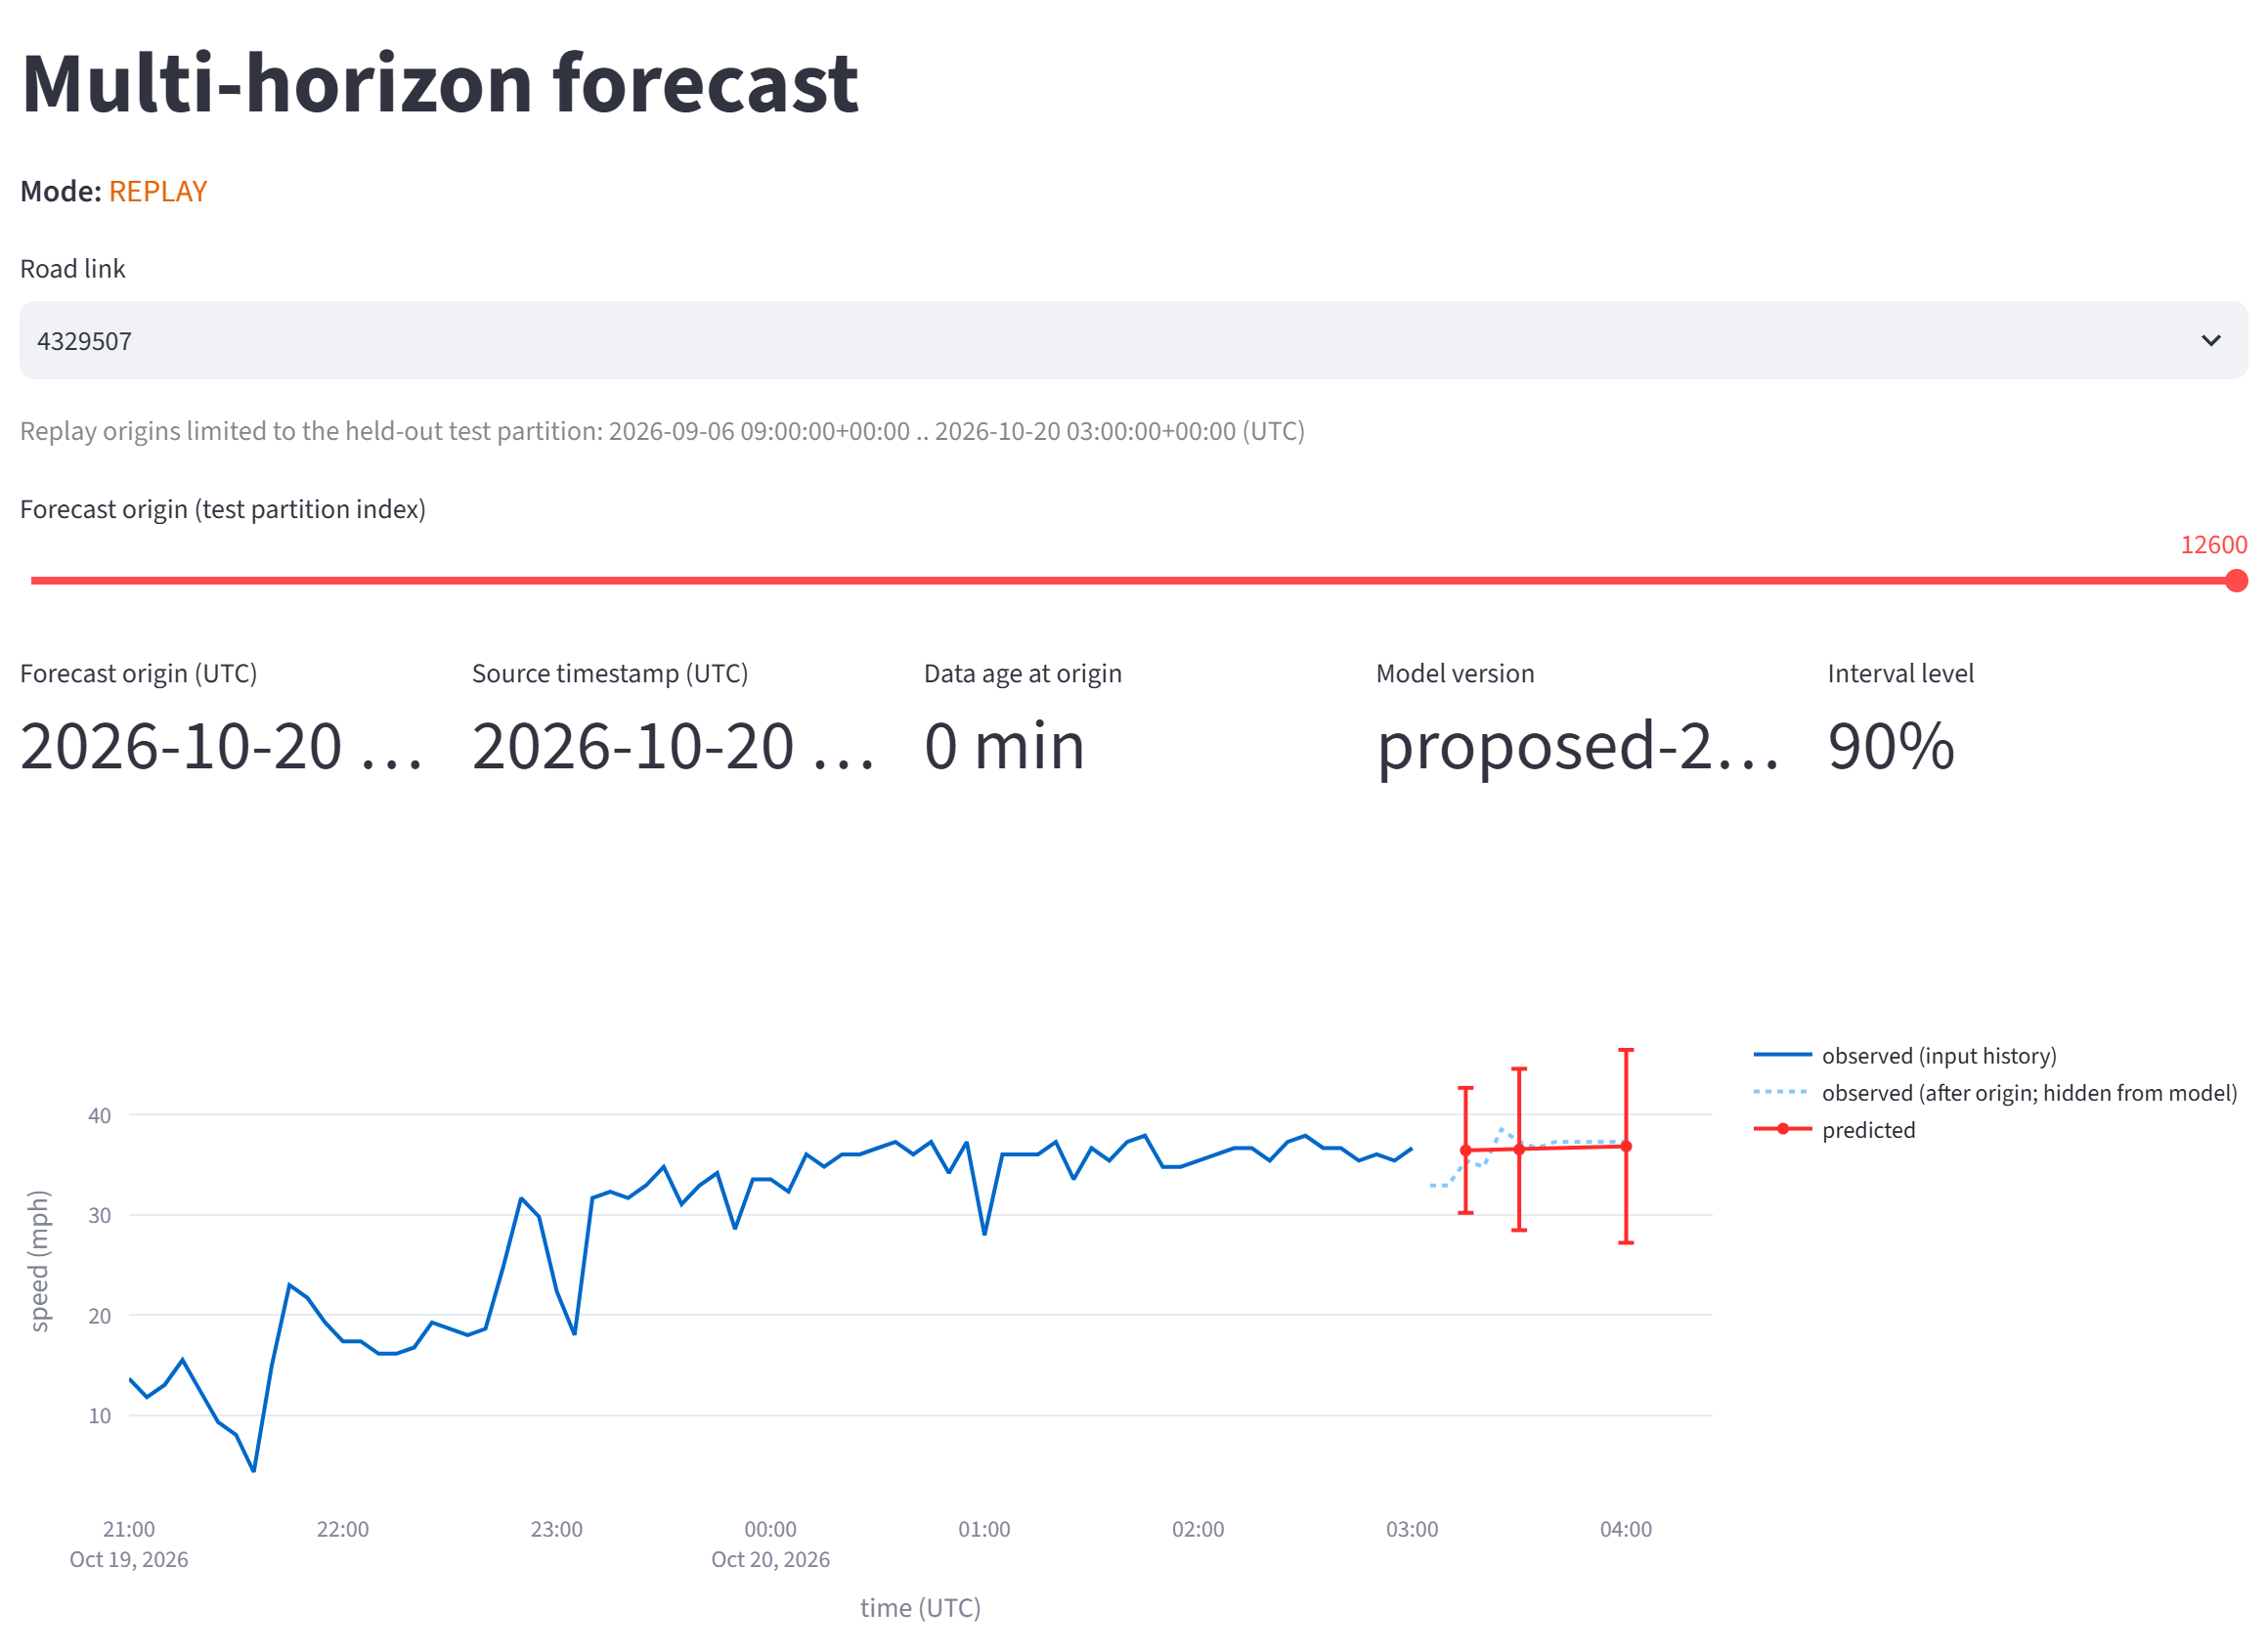
\includegraphics[width=0.810\textwidth]{fig14_dash_forecast.png}
\caption{Multi-horizon forecast page of the dashboard (REPLAY): the observed speed of one link with the 15, 30 and 60 minute forecasts and their 90\% intervals.}
\label{fig:dash}
\end{figure*}

The dashboard (Fig.~\ref{fig:dash}) shows each forecast with its interval, data age and mode label, and lists every advisory with its decision and reasons. On a CPU, one forecast for all links takes 5.7 ms with the proposed model, 2.2 ms with the temporal Transformer and 0.7 ms with the GRU (Table~\ref{tab:runtime}), a grouped explanation takes a few seconds per alert and a retrieval query takes tens of milliseconds. The language-model step dominates the latency of an advisory, which is acceptable for monitor-only advice but would need attention for faster control loops.

\begin{table}[!t]
\caption{Inference Time on a CPU}
\label{tab:runtime}
\centering\footnotesize
\setlength{\tabcolsep}{3pt}
\renewcommand{\arraystretch}{1.08}
\begin{tabular}{>{\raggedright\arraybackslash}p{\dimexpr 0.6712\columnwidth-2\tabcolsep\relax}>{\raggedleft\arraybackslash}p{\dimexpr 0.3288\columnwidth-2\tabcolsep\relax}}
\toprule
\textbf{Component} & \textbf{Time} \\
\midrule
Proposed & 5.693 ms \\
Temporal Transf. & 2.156 ms \\
GRU & 0.679 ms \\
LightGBM & 0.386 ms \\
XGBoost & 0.081 ms \\
Historical average & 0.9 µs \\
Persistence & 0.6 µs \\
\multicolumn{2}{@{}l@{}}{\emph{Explanation and retrieval}} \\
Grouped KernelSHAP, per alert & 1.7--4.2 s \\
Retrieval query (median) & 28 ms \\
\bottomrule
\end{tabular}
\par\vspace{2pt}
\begin{minipage}{\columnwidth}\scriptsize Forecast times are per origin; one origin covers all modelled links and three horizons. Retrieval median excludes the first query, which loads the encoder.\end{minipage}
\end{table}

\subsection{Discussion}
Three lessons stand out. First, graph structure helps, but modestly: the graph layers beat a temporal Transformer reliably, yet a GRU stays within a few hundredths of a mph. Second, calibration in aggregate hides failure in the tail; coverage drops below 0.80 in congestion, which argues for state-dependent or adaptive intervals \cite{gibbs2021aci,barber2023beyond}. Third, the most useful parts of the advisory are the deterministic ones. Retrieval stopped invented citations, and the constraint layer caught an advisory that retrieval alone let through. The live test shows that accuracy on held-out history does not guarantee value on a delayed feed, and that a fair live comparison must keep persistence in view.

\section{Limitations}\label{sec:limits}
The study covers 13 evaluated links in one borough over one test period, so the results may not transfer to other networks or seasons. The open speed feed is delayed and patchy, with half of the raw records carrying no measurement. The intervals assume exchangeability, which traffic violates, and they under-cover congestion. Explanations cover twelve alerts and describe the model, not causes on the street. Retrieval labels were reviewed by the first author only. The simulation testbed is calibrated to one observed speed, has no side-street demand or pedestrians and uses assumed timing plans, so its gains are illustrative. The live test spans three afternoons and nine batches. Finally, nothing was deployed on real signals, and every advisory stops at human review.

\section{Conclusion and Future Work}\label{sec:concl}
We built and tested an auditable system that forecasts city traffic from open data and turns reliable alerts into checked advice. The context-gated graph transformer cut forecast error against persistence by 7\% to 16\% on held-out data and beat a temporal Transformer at every horizon, but it was only marginally better than a GRU. Conformal intervals with a reliability gate made the forecasts safer to act on, although they covered congested periods too rarely. Grouped Shapley values produced explanations that an operator can read, and they agreed with the ablations. The language model, held in place by retrieval, deterministic rules and a calibrated simulation gate, gave valid, cited and cautious advisories, and a forecast-triggered rule reduced simulated delay by about 5\% under stress. On the live feed, at its present delay, the model did not beat persistence at short horizons.

Future work will add state-dependent and adaptive conformal intervals, test on more links and longer live periods with a lower-latency feed, include side-street and pedestrian demand in the testbed, and invite independent reviewers to label retrieval queries and judge advisories.

\balance
\begin{thebibliography}{40}
\bibitem{ji2023hallucination} Z. Ji \emph{et al.}, ``Survey of hallucination in natural language generation,'' \emph{ACM Comput. Surv.}, vol. 55, no. 12, pp. 1--38, 2023, doi: 10.1145/3571730.
\bibitem{vlahogianni2014shortterm} E. I. Vlahogianni, M. G. Karlaftis, and J. C. Golias, ``Short-term traffic forecasting: Where we are and where we're going,'' \emph{Transp. Res. Part C: Emerg. Technol.}, vol. 43, pp. 3--19, 2014, doi: 10.1016/j.trc.2014.01.005.
\bibitem{jiang2022gnnsurvey} W. Jiang and J. Luo, ``Graph neural network for traffic forecasting: A survey,'' \emph{Expert Syst. Appl.}, vol. 207, Art. no. 117921, 2022, doi: 10.1016/j.eswa.2022.117921.
\bibitem{lv2014bigdata} Y. Lv, Y. Duan, W. Kang, Z. Li, and F.-Y. Wang, ``Traffic flow prediction with big data: A deep learning approach,'' \emph{IEEE Trans. Intell. Transp. Syst.}, 2014, doi: 10.1109/TITS.2014.2345663.
\bibitem{ma2015lstm} X. Ma, Z. Tao, Y. Wang, H. Yu, and Y. Wang, ``Long short-term memory neural network for traffic speed prediction using remote microwave sensor data,'' \emph{Transp. Res. Part C: Emerg. Technol.}, vol. 54, pp. 187--197, 2015, doi: 10.1016/j.trc.2015.03.014.
\bibitem{cho2014gru} K. Cho \emph{et al.}, ``Learning phrase representations using RNN encoder--decoder for statistical machine translation,'' in \emph{Proc. Conf. Empirical Methods Natural Lang. Process. (EMNLP)}, 2014, pp. 1724--1734, doi: 10.3115/v1/D14-1179.
\bibitem{chen2016xgboost} T. Chen and C. Guestrin, ``XGBoost: A scalable tree boosting system,'' in \emph{Proc. 22nd ACM SIGKDD Int. Conf. Knowl. Discovery Data Mining}, 2016, pp. 785--794, doi: 10.1145/2939672.2939785.
\bibitem{ke2017lightgbm} G. Ke \emph{et al.}, ``LightGBM: A highly efficient gradient boosting decision tree,'' in \emph{Advances in Neural Information Processing Systems}, vol. 30, 2017.
\bibitem{li2018dcrnn} Y. Li, R. Yu, C. Shahabi, and Y. Liu, ``Diffusion convolutional recurrent neural network: Data-driven traffic forecasting,'' in \emph{Proc. Int. Conf. Learn. Represent. (ICLR)}, 2018, arXiv:1707.01926.
\bibitem{yu2018stgcn} B. Yu, H. Yin, and Z. Zhu, ``Spatio-temporal graph convolutional networks: A deep learning framework for traffic forecasting,'' in \emph{Proc. Int. Joint Conf. Artif. Intell. (IJCAI)}, 2018, pp. 3634--3640, doi: 10.24963/ijcai.2018/505.
\bibitem{wu2019graphwavenet} Z. Wu, S. Pan, G. Long, J. Jiang, and C. Zhang, ``Graph WaveNet for deep spatial-temporal graph modeling,'' in \emph{Proc. Int. Joint Conf. Artif. Intell. (IJCAI)}, 2019, pp. 1907--1913, doi: 10.24963/ijcai.2019/264.
\bibitem{bai2020agcrn} L. Bai, L. Yao, C. Li, X. Wang, and C. Wang, ``Adaptive graph convolutional recurrent network for traffic forecasting,'' 2020, arXiv:2007.02842.
\bibitem{guo2019astgcn} S. Guo, Y. Lin, N. Feng, C. Song, and H. Wan, ``Attention based spatial-temporal graph convolutional networks for traffic flow forecasting,'' in \emph{Proc. AAAI Conf. Artif. Intell.}, vol. 33, no. 1, 2019, pp. 922--929, doi: 10.1609/aaai.v33i01.3301922.
\bibitem{zheng2020gman} C. Zheng, X. Fan, C. Wang, and J. Qi, ``GMAN: A graph multi-attention network for traffic prediction,'' in \emph{Proc. AAAI Conf. Artif. Intell.}, vol. 34, no. 1, 2020, pp. 1234--1241, doi: 10.1609/aaai.v34i01.5477.
\bibitem{velickovic2017gat} P. Veličković, G. Cucurull, A. Casanova, A. Romero, P. Liò, and Y. Bengio, ``Graph attention networks,'' 2017, arXiv:1710.10903.
\bibitem{brody2022gatv2} S. Brody, U. Alon, and E. Yahav, ``How attentive are graph attention networks?'' in \emph{Proc. Int. Conf. Learn. Represent. (ICLR)}, 2022, arXiv:2105.14491.
\bibitem{vaswani2017attention} A. Vaswani \emph{et al.}, ``Attention is all you need,'' in \emph{Advances in Neural Information Processing Systems}, vol. 30, 2017, pp. 5998--6008.
\bibitem{vovk2005algorithmic} V. Vovk, A. Gammerman, and G. Shafer, \emph{Algorithmic Learning in a Random World}. New York, NY, USA: Springer, 2005, doi: 10.1007/b106715.
\bibitem{angelopoulos2021gentle} A. N. Angelopoulos and S. Bates, ``A gentle introduction to conformal prediction and distribution-free uncertainty quantification,'' 2021, arXiv:2107.07511.
\bibitem{xu2021enbpi} C. Xu and Y. Xie, ``Conformal prediction interval for dynamic time-series,'' in \emph{Proc. 38th Int. Conf. Mach. Learn. (ICML)}, PMLR, vol. 139, 2021, pp. 11559--11569.
\bibitem{gibbs2021aci} I. Gibbs and E. Candès, ``Adaptive conformal inference under distribution shift,'' 2021, arXiv:2106.00170.
\bibitem{barber2023beyond} R. F. Barber, E. J. Candès, A. Ramdas, and R. J. Tibshirani, ``Conformal prediction beyond exchangeability,'' \emph{Ann. Statist.}, vol. 51, no. 2, pp. 816--845, 2023, doi: 10.1214/23-AOS2276.
\bibitem{ribeiro2016lime} M. T. Ribeiro, S. Singh, and C. Guestrin, ```Why should I trust you?': Explaining the predictions of any classifier,'' in \emph{Proc. 22nd ACM SIGKDD Int. Conf. Knowl. Discovery Data Mining}, 2016, pp. 1135--1144, doi: 10.1145/2939672.2939778.
\bibitem{lundberg2017shap} S. M. Lundberg and S.-I. Lee, ``A unified approach to interpreting model predictions,'' in \emph{Advances in Neural Information Processing Systems}, vol. 30, 2017, arXiv:1705.07874.
\bibitem{lundberg2020treeshap} S. M. Lundberg \emph{et al.}, ``From local explanations to global understanding with explainable AI for trees,'' \emph{Nat. Mach. Intell.}, vol. 2, no. 1, pp. 56--67, 2020, doi: 10.1038/s42256-019-0138-9.
\bibitem{lewis2020rag} P. Lewis \emph{et al.}, ``Retrieval-augmented generation for knowledge-intensive NLP tasks,'' in \emph{Advances in Neural Information Processing Systems}, vol. 33, 2020, arXiv:2005.11401.
\bibitem{reimers2019sbert} N. Reimers and I. Gurevych, ``Sentence-BERT: Sentence embeddings using Siamese BERT-networks,'' in \emph{Proc. EMNLP-IJCNLP}, 2019, pp. 3982--3992, doi: 10.18653/v1/D19-1410.
\bibitem{johnson2019faiss} J. Johnson, M. Douze, and H. Jégou, ``Billion-scale similarity search with GPUs,'' \emph{IEEE Trans. Big Data}, vol. 7, no. 3, pp. 535--547, 2021, doi: 10.1109/TBDATA.2019.2921572.
\bibitem{yao2023react} S. Yao \emph{et al.}, ``ReAct: Synergizing reasoning and acting in language models,'' in \emph{Proc. Int. Conf. Learn. Represent. (ICLR)}, 2023, arXiv:2210.03629.
\bibitem{fhwa2008stm} P. Koonce \emph{et al.}, ``Traffic signal timing manual,'' U.S. Dept. of Transportation, Federal Highway Administration, Washington, DC, USA, Rep. FHWA-HOP-08-024, 2008.
\bibitem{mutcd2009} U.S. Dept. of Transportation, Federal Highway Administration, \emph{Manual on Uniform Traffic Control Devices for Streets and Highways}, 2009 ed. Washington, DC, USA, 2009.
\bibitem{wei2018intellilight} H. Wei, G. Zheng, H. Yao, and Z. Li, ``IntelliLight: A reinforcement learning approach for intelligent traffic light control,'' in \emph{Proc. 24th ACM SIGKDD Int. Conf. Knowl. Discovery Data Mining}, 2018, pp. 2496--2505, doi: 10.1145/3219819.3220096.
\bibitem{lopez2018sumo} P. A. Lopez \emph{et al.}, ``Microscopic traffic simulation using SUMO,'' in \emph{Proc. 21st IEEE Int. Conf. Intell. Transp. Syst. (ITSC)}, 2018, pp. 2575--2582, doi: 10.1109/ITSC.2018.8569938.
\bibitem{nycdotspeeds} New York City Department of Transportation, ``DOT traffic speeds NBE,'' NYC Open Data, dataset i4gi-tjb9. Accessed: Oct. 20, 2026. [Online]. Available: \url{https://data.cityofnewyork.us/d/i4gi-tjb9}
\bibitem{openmeteo} Open-Meteo, ``Historical weather and historical forecast APIs,'' CC BY 4.0. Accessed: Oct. 20, 2026. [Online]. Available: \url{https://open-meteo.com}
\bibitem{nycclasscounts} New York City Department of Transportation, ``Vehicle classification counts (2011--2025),'' NYC Open Data, dataset 96ay-ea4r. Accessed: Oct. 21, 2026.
\bibitem{fey2019pyg} M. Fey and J. E. Lenssen, ``Fast graph representation learning with PyTorch Geometric,'' presented at the ICLR Workshop Represent. Learn. Graphs Manifolds, 2019, arXiv:1903.02428.
\bibitem{rozemberczki2021pgt} B. Rozemberczki \emph{et al.}, ``PyTorch Geometric Temporal: Spatiotemporal signal processing with neural machine learning models,'' in \emph{Proc. 30th ACM Int. Conf. Inf. Knowl. Manage. (CIKM)}, 2021, pp. 4564--4573, doi: 10.1145/3459637.3482014.
\bibitem{nycvzvretiming} New York City Department of Transportation, ``VZV signal timing / 25 MPH signal retiming,'' NYC Open Data, dataset d8dp-wfee. Accessed: Oct. 21, 2026.
\bibitem{sumodocs_routing} Eclipse SUMO contributors, ``Automatic routing / routing device (SUMO 1.28.0 documentation),'' section ``Incomplete trips and flows,'' 2026. Accessed: Oct. 21, 2026. [Online]. Available: \url{https://github.com/eclipse-sumo/sumo/blob/v1_28_0/docs/web/docs/Demand/Automatic_Routing.md}
\end{thebibliography}
\end{document}
